% Template for PLoS
% Version 3.1 February 2015
%
% To compile to pdf, run:
% latex plos.template
% bibtex plos.template
% latex plos.template
% latex plos.template
% dvipdf plos.template
%
% % % % % % % % % % % % % % % % % % % % % %
%
% -- IMPORTANT NOTE
%
% This template contains comments intended
% to minimize problems and delays during our production
% process. Please follow the template instructions
% whenever possible.
%
% % % % % % % % % % % % % % % % % % % % % % %
%
% Once your paper is accepted for publication,
% PLEASE REMOVE ALL TRACKED CHANGES in this file and leave only
% the final text of your manuscript.
%
% There are no restrictions on package use within the LaTeX files except that
% no packages listed in the template may be deleted.
%
% Please do not include colors or graphics in the text.
%
% Please do not create a heading level below \subsection. For 3rd level headings, use \paragraph*{}.
%
% % % % % % % % % % % % % % % % % % % % % % %
%
% -- FIGURES AND TABLES
%
% Please include tables/figure captions directly after the paragraph where they are first cited in the text.
%
% DO NOT INCLUDE GRAPHICS IN YOUR MANUSCRIPT
% - Figures should be uploaded separately from your manuscript file.
% - Figures generated using LaTeX should be extracted and removed from the PDF before submission.
% - Figures containing multiple panels/subfigures must be combined into one image file before submission.
% For figure citations, please use "Fig." instead of "Figure".
% See http://www.plosone.org/static/figureGuidelines for PLOS figure guidelines.
%
% Tables should be cell-based and may not contain:
% - tabs/spacing/line breaks within cells to alter layout or alignment
% - vertically-merged cells (no tabular environments within tabular environments, do not use \multirow)
% - colors, shading, or graphic objects
% See http://www.plosone.org/static/figureGuidelines#tables for table guidelines.
%
% For tables that exceed the width of the text column, use the adjustwidth environment as illustrated in the example table in text below.
%
% % % % % % % % % % % % % % % % % % % % % % % %
%
% -- EQUATIONS, MATH SYMBOLS, SUBSCRIPTS, AND SUPERSCRIPTS
%
% IMPORTANT
% Below are a few tips to help format your equations and other special characters according to our specifications. For more tips to help reduce the possibility of formatting errors during conversion, please see our LaTeX guidelines at http://www.plosone.org/static/latexGuidelines
%
% Please be sure to include all portions of an equation in the math environment.
%
% Do not include text that is not math in the math environment. For example, CO2 will be CO\textsubscript{2}.
%
% Please add line breaks to long display equations when possible in order to fit size of the column.
%
% For inline equations, please do not include punctuation (commas, etc) within the math environment unless this is part of the equation.
%
% % % % % % % % % % % % % % % % % % % % % % % %
%
% Please contact latex@plos.org with any questions.
%
% % % % % % % % % % % % % % % % % % % % % % % %

\documentclass[10pt,letterpaper]{article}
\usepackage[top=0.85in,left=2.75in,footskip=0.75in]{geometry}

% Use adjustwidth environment to exceed column width (see example table in text)
\usepackage{changepage}

% Use Unicode characters when possible
%\usepackage[utf8]{inputenc}

% textcomp package and marvosym package for additional characters
\usepackage{textcomp,marvosym}

% fixltx2e package for \textsubscript
\usepackage{fixltx2e}

% amsmath and amssymb packages, useful for mathematical formulas and symbols
\usepackage{amsmath,amssymb}

% cite package, to clean up citations in the main text. Do not remove.
\usepackage{cite}

% Use nameref to cite supporting information files (see Supporting Information section for more info)
\usepackage{nameref}
\usepackage{color}
\usepackage[colorlinks=true,
            linkcolor=blue,
            urlcolor=blue,
            citecolor=black]{hyperref}


% line numbers
\usepackage[right]{lineno}

% ligatures disabled
\usepackage{microtype}
\DisableLigatures[f]{encoding = *, family = * }

% rotating package for sideways tables
\usepackage{rotating}

% Remove comment for double spacing
%\usepackage{setspace}
%\doublespacing

\usepackage{graphicx}
\usepackage[space]{grffile}
\usepackage{latexsym}
\usepackage{textcomp}
\usepackage{longtable}
\usepackage{multirow,booktabs}
% You can conditionalize code for latexml or normal latex using this.
\newif\iflatexml\latexmlfalse
\usepackage[utf8]{inputenc}
\usepackage[ngerman,greek,english]{babel}

%% Neutralize any \includegraphics in the document, as PLOS does not allow figures in the final submission
\makeatletter
\let\orig@includegraphics\includegraphics
\AtBeginDocument{\let\includegraphics\PLOS@ignore}
\newcommand{\PLOS@ignore}[2][]{}
\makeatother



% Text layout
\raggedright
\setlength{\parindent}{0.5cm}
\textwidth 5.25in
\textheight 8.75in

% Bold the 'Figure #' in the caption and separate it from the title/caption with a period
% Captions will be left justified
\usepackage[aboveskip=1pt,labelfont=bf,labelsep=period,justification=raggedright,singlelinecheck=off]{caption}

% Use the PLoS provided BiBTeX style
\bibliographystyle{plos2015}

% Remove brackets from numbering in List of References
\makeatletter
\renewcommand{\@biblabel}[1]{\quad#1.}
\makeatother

% Leave date blank
\date{}

% Header and Footer with logo
\usepackage{lastpage,fancyhdr,graphicx}
\usepackage{epstopdf}
\pagestyle{myheadings}
\pagestyle{fancy}
\fancyhf{}
\makeatletter
\lhead{\orig@includegraphics[width=2.0in]{PLOS-submission.eps}}
\makeatother
\rfoot{\thepage/\pageref{LastPage}}
\renewcommand{\footrule}{\hrule height 2pt \vspace{2mm}}
\fancyheadoffset[L]{2.25in}
\fancyfootoffset[L]{2.25in}
\lfoot{\sf PLOS}

%% Include all macros below

\newcommand{\lorem}{{\bf LOREM}}
\newcommand{\ipsum}{{\bf IPSUM}}

\usepackage{color}
\usepackage{listings}
\lstset{ %
  backgroundcolor=\color{white},   % choose the background color
  basicstyle=\footnotesize\ttfamily,        % size of fonts used for the code
  breaklines=true,                 % automatic line breaking only at whitespace
  captionpos=b,                    % sets the caption-position to bottom
  commentstyle=\color{OliveGreen},    % comment style
  keywordstyle=\color{blue},       % keyword style
  stringstyle=\color{black},     % string literal style
  language=Python,             % Set your language (you can change the language for each code-block optionally)
  frame=l, %
  xleftmargin=\fboxsep, %
  xrightmargin=-\fboxsep, %
}
\hyphenation{smFRET}
\hyphenation{FRETBursts}

%% END MACROS SECTION


\begin{document}
\vspace*{0.35in}

% Title must be 250 characters or less.
\begin{flushleft}
{\Large
\textbf\newline{FRETBursts: An Open Source Toolkit for the Analysis of FRET in Single-Molecules Diffusing in Solution
}
}
\newline
% Insert author names, affiliations and corresponding author email (do not include titles, positions, or degrees).
\\
Antonino Ingargiola\textsuperscript{1*},
Eitan Lerner\textsuperscript{1},
SangYoon Chung\textsuperscript{1},
Shimon Weiss\textsuperscript{1},
Xavier Michalet\textsuperscript{1},
\\
\bigskip
\textbf{1} Dept. Chemistry and Biochemistry, Univ. of California Los Angeles, Los Angeles, CA, USA
\bigskip

% Use the asterisk to denote corresponding authorship and provide email address in note below.
* ingargiola.antonino@gmail.com
\end{flushleft}

% Please keep the abstract below 300 words

\section*{Abstract}
Single-molecule Förster Resonance Energy Transfer (smFRET) allows
probing intermolecular interactions and conformational changes in
biomacromolecules, and represents an invaluable tool for studying
cellular processes at the molecular scale. smFRET experiments can
detect the distance between two fluorescent labels (donor and acceptor)
in the 3-10~nm range. In the commonly employed confocal geometry,
molecules are free to diffuse in solution. When a molecule traverses
the excitation volume, it emits a burst of photons, which can be detected
by single-photon avalanche diode (SPAD) detectors. The intensities of
donor and acceptor fluorescence can then be related to the distance
between the two fluorophores.

While recent years have seen a growing number of contributions
proposing improvements or new techniques in smFRET data analysis,
rarely have those publications been accompanied by software implementation.
In particular, despite the widespread application of smFRET, no complete
software package for smFRET burst analysis is freely available to date.

In this paper, we introduce FRETBursts, an open source software
for analysis of freely-diffusing smFRET data.
FRETBursts allows executing all the fundamental steps of smFRET bursts
analysis using state-of-the-art as well as novel techniques,
while providing an open, robust and well-documented implementation.
Therefore, FRETBursts represents an ideal platform for comparison
and development of new methods in burst analysis.

We employ modern software engineering principles in order to
minimize bugs and facilitate long-term maintainability.
Furthermore, we place a strong focus on reproducibility by relying on
Jupyter notebooks for FRETBursts execution.
Notebooks are executable documents capturing all the steps of the
analysis (including data files, input parameters, and results) and can
be easily shared to replicate complete smFRET analyzes.
Notebooks allow beginners to execute complex workflows
and advanced users to customize the analysis for their own needs.
By bundling analysis description, code and results in a single document,
FRETBursts allows to seamless share analysis workflows
and results, encourages reproducibility and facilitates collaboration
among researchers in the single-molecule community.


% Please keep the Author Summary between 150 and 200 words
% Use first person. PLOS ONE authors please skip this step.
% Author Summary not valid for PLOS ONE submissions.
%\section*{Author Summary}

\linenumbers



\section*{Introduction}

\subsection*{Open Science and Reproducibility}

Over the past 20 years, single molecule FRET (smFRET) has grown into one of the most
useful techniques in single-molecule spectroscopy~\cite{Weiss_1999,Hohlbein_2014}.
While it is possible to extract information on sub-populations using ensemble measurements
(e.g. ~\cite{Lerner_2014,Rahamim_2015}),
smFRET unique feature is its ability to very straightforwardly resolve conformational
changes of biomolecules or measure binding-unbinding kinetics in heterogeneous
samples~\cite{Selvin_2000,Roy_2008,Schuler_2008,Sisamakis_2010,Haran_2012}.
smFRET measurements on freely diffusing molecules (the focus of this paper)
have the additional advantage, over measurements performed on immobilized molecules,
of allowing to probe molecules and processes without perturbation from surface
immobilization or additional functionalization needed for surface
attachment~\cite{Eggeling_1998,Dahan_1999}.

The increasing amount of work using freely-diffusing smFRET has motivated
a growing number of theoretical contributions to the specific topic of data
analysis~\cite{Fries_1998,Eggeling_2001,Zhang_2005,Gopich_2005,Lee_2005,Nir_2006,Antonik2006,Gopich_2007,Gopich_2008,Camley_2009,Santoso_2010,Torella_2011,Tomov_2012}.
Despite this profusion of publications, most research groups still rely on
their own implementation of a limited number of methods, with very little
collaboration or code sharing.
To clarify this statement, let us point that our own group's past smFRET papers
merely mention the use of custom-made software without additional details~\cite{Lee_2005,Nir_2006}.
Even though some of these software tools are made available upon request,
or sometimes shared publicly on websites,
it remains hard to reproduce and validate results from different groups,
let alone build upon them.
Additionally, as new methods are proposed in literature,
it is generally difficult to quantify their performance compared to other methods.
An independent quantitative assessment
would require a complete reimplementation, an effort few groups can afford.
As a result, potentially useful analysis improvements
are either rarely or slowly adopted by the community.
In contrast with other established traditions such as
sharing protocols and samples, in the domain of scientific software,
we have relegated ourselves to islands of non-communication.

From a more general standpoint, the non-availability of the code
used to produce scientific results, hinders reproducibility,
makes it impossible to review and validate the software's correctness
and prevents improvements and extensions by other scientists.
This situation, common in many disciplines,
represents a real impediment to the scientific progress.
Since the pioneering work of the Donoho group in the 90's~\cite{Buckheit_1995},
it has become evident that developing and maintaining open source scientific software
for reproducible research is a critical requirement of the modern
scientific enterprise~\cite{Ince_2012,Vihinen_2015}.

%Peer-reviewed publications describing such software are also necessary~\cite{Pradal_2013},
%although the debate is still open on the most effective model for peer-reviewing this
%class of publications~\cite{Check_Hayden_2013,Check_Hayden_2015}
%(\href{https://software-carpentry.org/blog/2015/04/quality-is-free-getting-there-isnt.html}{Willson 2015})
%(\href{https://www.mozillascience.org/effective-code-review-for-journals}{Mills 2015})
%(\href{http://ivory.idyll.org/blog/2015-we-live-in-a-bubble.html}{Brown 2015} and \href{http://ivory.idyll.org/blog/on-code-review-of-scientific-code.html}{2013}).

Other disciplines have started tackling this issue~\cite{Eglen_2016},
and even in the single-molecule field a few recent publications have provided
software for analysis of surface-immobilized experiments~\cite{McKinney_2006,Bronson_2009,Greenfeld_2012,K_nig_2013,van_de_Meent_2014}.
For freely-diffusing smFRET experiments, although it is common to find mention of
``code available from the authors upon reques'' in publications, there is a dearth
of such open source code, with, to our knowledge, the notable exception of a single
example~\cite{Murphy2014}.
To address this issue, we have developed FRETBursts,
an open source Python software for analysis of freely-diffusing single-molecule FRET measurements.
FRETBursts can be used, inspected and modified by anyone interested in using
state-of-the art smFRET analysis methods or implementing modifications or completely new techniques.
FRETBursts therefore represents an ideal platform
for quantitative comparison of different methods for smFRET burst analysis.
Technically, a strong emphasis has been given to the reproducibility of complete analysis
workflows. FRETBursts uses Jupyter Notebooks~\cite{Shen_2014},
an interactive and executable document containing textual narrative, input parameters,
code, and computational results (tables, plots, etc.). A notebook thus captures the various analysis steps
in a document which is easy to share and execute.
To minimize the possibility of bugs being introduced inadvertently~\cite{Soergel_2015},
we employ modern software engineering techniques
such as unit testing and continuous integration~\cite{Wilson_2014,Eglen_2016}.
FRETBursts is hosted on GitHub~\cite{Blischak_2016,Prli__2012},
where users can write comments, report issues or contribute code.
In a related effort, we recently introduced Photon-HDF5~\cite{Ingargiola2016},
an open file format for timestamp-based single-molecule fluorescence
experiments. An other related open source tool is PyBroMo~\cite{Ingargiola_2016},
a freely-diffusing smFRET simulator which produces Photon-HDF5 files that are
directly analyzable with FRETBursts.
Together with all the aforementioned tools, FRETBursts contributes to the growing
ecosystem of open tools for reproducible science in the single-molecule field.

\subsection*{Paper Overview}
This paper is written as an introduction to smFRET burst analysis and
its implementation in FRETBursts.
The aim is illustrating the specificities and
trade-offs involved in various approaches
with sufficient details to enable readers
to customize the analysis for their own needs.

After a brief overview of FRETBursts features (section~\nameref{sec:overview}),
we introduce essential concepts and terminology for smFRET burst analysis
(section~\nameref{sec:concepts}).
In section~\nameref{sec:analysis}, we illustrate the steps involved
in smFRET burst analysis: (i) data loading (section~\nameref{sec:dataload}),
(ii) definition of the excitation alternation periods
(section~\nameref{sec:alternation}), (iii) background correction
(section~\nameref{sec:bg_calc}), (iv) burst search
(section~\nameref{sec:burstsearch}),
(v) burst selection (section~\nameref{sec:burstsel}) and
(vi) FRET histogram fitting (section~\nameref{sec:fretfit}).
As an example
of implementation of an advanced data processing technique,
section~\nameref{sec:bva} walks the reader thorough implementing
Burst Variance Analysis (BVA)~\cite{Torella_2011}.
Finally, section~\nameref{sec:conclusions} summarizes what we believe
to be the strengths of FRETBursts software.

Throughout this paper,
links to relevant sections of documentation and other web resources
are displayed as ``(link)''.
In order to make the text more legible,
we have concentrated Python-specific details in paragraphs titled
\textit{Python details}. These subsections provide deeper insights for readers
already familiar with Python and can be initially skipped by readers who are not.
Finally, note that all commands and figures in this paper can be regenerated
using the accompanying notebooks
(\href{https://github.com/tritemio/fretbursts_paper}{link}).


\section*{FRETBursts Overview}
\label{sec:overview}

\subsection*{Technical Features}

FRETBursts can analyze smFRET measurements
from one or multiple excitation spots~\cite{Ingargiola_2013}. The supported
excitation schemes include single laser, alternating laser excitation (ALEX)
with either CW lasers (μs-ALEX~\cite{Kapanidis_2005})
or pulsed lasers (ns-ALEX~\cite{Laurence_2005} or
pulsed-interleaved excitation (PIE)~\cite{M_ller_2005}).

The software implements both standard and novel algorithms for smFRET data analysis
including background estimation as a function of time (including background accuracy
metrics), sliding-window burst search~\cite{Eggeling_1998},
dual-channel burst search (DCBS)~\cite{Nir_2006} and
modular burst selection methods based on user-defined criteria
(including a large set of pre-defined selection rules). Novel features include burst size
selection with $\gamma$-corrected burst sizes, burst weighting, burst search with
background-dependent threshold (in order to guarantee a minimal signal-to-background
ratio~\cite{Michalet_2012}).
Moreover, FRETBursts provides a large set of fitting options to characterize FRET subpopulations.
In particular, distributions of burst quantities (such as $E$ or $S$) can be assessed
through (1) histogram fitting (with arbitrary model functions),
(2) non-parametric weighted kernel density estimation (KDE), (3) weighted
expectation-maximization (EM), (4) maximum likelihood fitting using Gaussian models
or Poisson statistic. Finally FRETBursts includes a large number of
predefined and customizable plot functions which (thanks to the \textit{matplotlib}
graphic library) produce publication quality plots in a wide range of formats.

Additionally, implementations of population dynamics analysis such
as Burst Variance Analysis (BVA)~\cite{Torella_2011} and two-channel
kernel density distribution estimator (2CDE)~\cite{Tomov_2012}
are available as FRETBursts notebooks
(\href{http://nbviewer.jupyter.org/github/tritemio/FRETBursts_notebooks/blob/master/notebooks/Example%20-%20Burst%20Variance%20Analysis.ipynb}{BVA link},
\href{http://nbviewer.jupyter.org/github/tritemio/FRETBursts_notebooks/blob/master/notebooks/Example%20-%202CDE%20Method.ipynb}{2CDE link}).

\subsection*{Software Availability}
FRETBursts is hosted and openly developed on GitHub. FRETBursts homepage
(\href{http://tritemio.github.io/FRETBursts}{link})
contains links to the various resources. Pre-built packages are provided for
Windows, OS X and Linux. Installation instructions
can be found in the Reference Documentation
(\href{http://fretbursts.readthedocs.org/en/latest/getting_started.html}{link}).
A description of FRETBursts execution using Jupyter notebooks is reported
in~\nameref{sec:notebook}. % SI_link
Detailed information on development style, testing strategies and
contributions guidelines are reported in~\nameref{sec:dev}. % SI_link
Finally, to facilitate evaluation and comparison with other software,
we set up an on-line services allowing to execute FRETBursts
without requiring any installation on the user's computer (\href{https://github.com/tritemio/FRETBursts_notebooks#run-online}{link}).


\section*{Architecture and Concepts}
\label{sec:concepts}

In this section, we introduce some general burst analysis concepts
and notations used in FRETBursts.

\subsection*{Photon Streams}
\label{sec:ph_streams}

The raw data collected during a smFRET experiment consists in one or more arrays of
photon timestamps, whose temporal resolution is set by the acquisition hardware,
typically between 10 and 50 ns.
In single-spot measurements, all timestamps are stored in a single array. In multispot
measurements~\cite{Ingargiola_2013}, there are as many timestamps arrays
as excitation spots.
Each array contains timestamps from both donor (D) and acceptor (A) channels.
When alternating excitation lasers are used (ALEX measurements)~\cite{Lee_2005},
a further distinction between photons emitted during the D or A excitation periods can be made.

In FRETBursts, the corresponding sets of photons are called ``photon streams'' and are
specified with a \verb|Ph_sel| object
(\href{http://fretbursts.readthedocs.org/en/latest/ph_sel.html}{link}).
In non-ALEX smFRET data, there are 3 photon streams
(table~\ref{tab:ph_sel_smfret}), while in ALEX data, there are 5 streams (table~\ref{tab:ph_sel_alex}).

The \verb|Ph_sel| class (\href{http://fretbursts.readthedocs.org/en/latest/ph_sel.html}{link})
allows the specification of any combination of photon streams.
For example, in ALEX measurements, the D-emission during A-excitation stream is
usually ignored because it does not contain any useful signal~\cite{Lee_2005}.
To indicate all but photons in this photon stream, the syntax is
\verb|Ph_sel(Dex='DAem', Aex='Aem')|, which indicates selection of donor
and acceptor photons (\verb|DAem|) during donor excitation (\verb|Dex|) and only acceptor
photons (\verb|Aem|) during acceptor excitation (\verb|Aex|).

\begin{table}
\begin{tabular}{l|l}
  Photon selection  & code \\
  \hline
  All-photons       & \verb|Ph_sel('all')|\\
  D-emission    & \verb|Ph_sel(Dex='Dem')|\\
  A-emission & \verb|Ph_sel(Dex='Aem')|\\
\end{tabular}
\caption{\label{tab:ph_sel_smfret}Photon selection syntax (non-ALEX)}
\end{table}

\begin{table}
\begin{tabular}{l|l}
  Photon selection  & code \\
  \hline
  All-photons & \verb|Ph_sel('all')|\\
  D-emission during D-excitation & \verb|Ph_sel(Dex='Dem')|\\
  A-emission during D-excitation & \verb|Ph_sel(Dex='Aem')|\\
  D-emission during A-excitation & \verb|Ph_sel(Aex='Dem')|\\
  A-emission during A-excitation & \verb|Ph_sel(Aex='Aem')|\\
\end{tabular}
\caption{\label{tab:ph_sel_alex}Photon selection syntax (ALEX)}
\end{table}

\subsection*{Background Definitions}
\label{sec:bg_intro}

An estimation of the background rates is needed to both select a proper threshold for
burst search, and to correct the raw burst counts by subtraction of background counts.

The recorded stream of timestamps is the result of two processes: one characterized
by a high count rate, due to fluorescence photons of single molecules crossing the
excitation volume, and another characterized by a lower count rate, due to ``background
counts'' originating from detector dark counts, afterpulsing, out-of-focus molecules
and sample scattering and/or impurities~\cite{Edman_1996,Gopich_2008}.
The signature of these two types of processes can be
observed in the inter-photon delays distribution (i.e. the waiting times
between two subsequent timestamps) as illustrated in figure~\ref{fig:bg_dist_all}(a).
The ``tail'' of the distribution (a straight line in semi-log scale) corresponds
to exponentially-distributed time-delays, indicating that those counts are generated by a
Poisson process. At short
timescales, the distribution departs from the exponential due to the contribution
of the higher rate process of single molecules traversing the excitation volume.
To estimate the background rate (i.e. the inverse of the exponential time constant),
it is necessary to define a time-delay threshold above which the distribution
can be considered exponential.
Finally, a parameter estimation method needs to be specified, such as Maximum
Likelihood Estimation (MLE) or non-linear least squares curve fitting of
the time-delay histogram (both supported in FRETBursts).


\begin{figure}[h!]
\begin{center}
\includegraphics[width=0.77\columnwidth]{figures/ph_delays_distrib_all/ph_delays_distrib_all}
\caption{\label{fig:bg_dist_all} \textbf{Inter-photon delays fitted with and exponential function.}
Experimental distributions of inter-photon delays (\textit{dots}) and
corresponding fits of the exponential tail (\textit{solid lines}).
(\textit{Panel a}) An example of inter-photon delays distribution (\textit{red dots}) and an exponential fit
of the tail of the distribution (\textit{black line}).
(\textit{Panel b}) Inter-photon delays distribution and exponential fit for different photon streams as obtained with \texttt{dplot(d, hist\_bg)}. The \textit{dots} represent the experimental histogram for the different photon streams. The \textit{solid lines} represent the corresponding exponential fit of the tail of the distributions. The legend shows abbreviations of the photon streams
and the fitted background rates.%
}
\end{center}
\end{figure}

It is advisable to monitor the background as a function of time
throughout the measurement, in order to account for possible variations.
Experimentally, we found that when the background is not constant,
it usually varies
on time scales of tens of seconds (see figure~\ref{fig:bg_timetrace}).
FRETBursts divides the acquisition in constant-duration time
windows called \textit{background periods} and computes the background rates for
each of these windows (see section~\nameref{sec:bg_calc}).
Note that FRETBursts uses these local background rates also during burst search,
in order to compute time-dependent burst detection thresholds
and for background correction of burst data (see section~\nameref{sec:burstsearch}).


\begin{figure}[h!]
\begin{center}
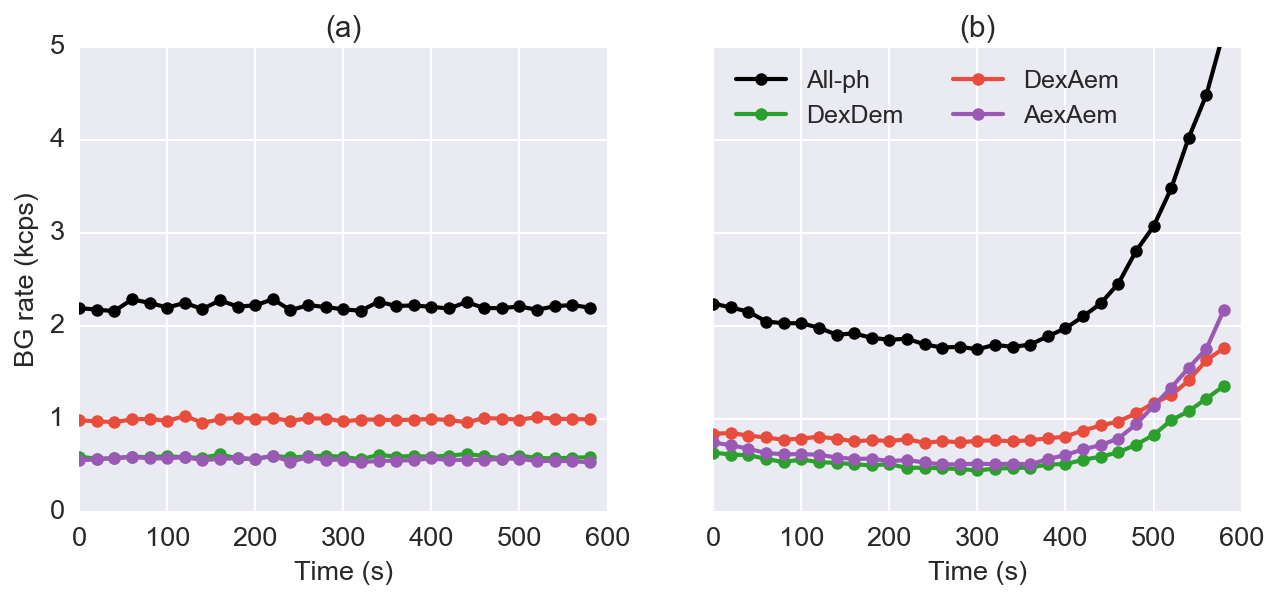
\includegraphics[width=0.91\columnwidth]{figures/background_timetrace/background_timetrace}
\caption{\label{fig:bg_timetrace} \textbf{Background rates as a function of time.}
Estimated background rate as a function of time for two μs-ALEX measurements.
Different colors represent different photon streams.
(\textit{Panel a}) A measurement performed with a sealed sample chamber
exhibiting constant a background as a function of time.
(\textit{Panel b}) A measurement performed on an unsealed sample exhibiting
significant background variations due to sample evaporation and/or
photobleaching (likely impurities on the cover-glass).
These plots are produced by the command
\texttt{dplot(d, timetrace\_bg)} after estimation of background.
Each data point in these figures is computed for a 30~s time window.%
}
\end{center}
\end{figure}


\subsection*{The \texttt{Data} Class}
\label{sec:data_intro}

The \verb|Data| class
(\href{http://fretbursts.readthedocs.org/en/latest/data_class.html}{link})
is the fundamental data container in FRETBursts. It contains the
measurement data and parameters (attributes) as well as several methods
for data analysis (background estimation, burst search, etc...).
All analysis results (bursts data, estimated parameters) are also stored
as \verb|Data| attributes.

There are 3 important ``burst counts'' attributes which contain
the number of photons detected in the donor or the acceptor channel
during donor or acceptor excitation (table~\ref{tab:data_n}).
The attributes in table~\ref{tab:data_n} are background-corrected by default.
Furthermore, \verb|na| is corrected for leakage and direct excitation
(section~\nameref{sec:corrcoeff}) if the relative coefficients are specified
(by default they are 0).
There is also a closely related attribute named \verb|nda| for donor photons
during acceptor excitation. \verb|nda| is normally neglected as it only contains
background.

\begin{table}
\begin{tabular}{l p{0.8\columnwidth}}
  Name  & Description \\
  \hline
  \verb|nd| & number of photons detected by the donor channel (during donor excitation period in ALEX case)\\
  \verb|na| & number of photons detected by the acceptor channel (during donor excitation period in ALEX case)\\
  \verb|naa| & number of photons detected by the acceptor channel during acceptor excitation period (present only in ALEX measurements)\\
\end{tabular}
\caption{\label{tab:data_n}\texttt{Data} attributes names and descriptions for burst photon counts in different photon streams.}
\end{table}


\paragraph*{Python details}
Many \verb|Data| attributes are lists of arrays (or scalars) with the length of the lists
equal to the number of excitation spots. This means that in
single-spot measurements, an array of burst-data
is accessed by specifying the index as 0, for example \verb|Data.nd[0]|.
\verb|Data| implements a shortcut syntax to access the first element of a list
with an underscore, so that an equivalently syntax is
\verb|Data.nd_| instead of \verb|Data.nd[0]|.

\subsection*{Introduction to Burst Search}
\label{sec:burstsearch_intro}

Identifying single-molecule fluorescence bursts in the stream of photons is
one of the most crucial steps in the analysis of freely-diffusing single-molecule FRET data.
The widely used ``sliding window'' algorithm, introduced by the Seidel group in
1998~\cite{Eggeling_1998,Fries_1998}, involves searching for
$m$ consecutive photons detected during a period shorter than
$\Delta t$. In other words, bursts are regions of the photon stream where the
local rate (computed using $m$ photons) is above a minimum threshold rate.
Since a universal criterion to choose the rate threshold and
the number of photons $m$ is, as of today, lacking, it has become a common
practice to manually adjust those parameters for each specific measurement.

A more general approach consists in taking into account the background rate of
the specific measurements and in choosing a rate threshold that is $F$ times
larger than the background rate. This approach ensures that all resulting bursts
have a signal-to-background ratio (SBR) larger than
$(F-1)$~\cite{Michalet_2012}. A consistent criterion for choosing the threshold is
particularly important when comparing different measurements with different background
rates, when the background significantly varies during measurements or in
multi-spot measurements where each spot has a different background rate.

A second important aspect of burst search is the choice of photon stream used
to perform the search.
In most cases, for instance when identifying FRET sub-populations,
the burst search should use all photons (i.e. APBS). In some other cases, when focusing on
donor-only or acceptor only populations, it is better to perform the search using
only donor or acceptor signal.
In order to handle the general case and to provide flexibility,
FRETBursts allows performing the burst search on arbitrary selections of photons.
(see section~\nameref{sec:ph_streams} for more information on photon stream definitions).

Additionally, Nir~\textit{et al.}~\cite{Nir_2006} proposed DCBS (``dual-channel burst search''), which can help mitigating artifacts due to photophysics effects such as blinking.
During DCBS, a search is performed in parallel on two photon streams
and bursts are defined as periods during which both photon streams exhibit a rate higher than
the threshold, implementing the equivalent of an AND logic operation.
Conventionally, the term DCBS refers to a burst search where the two photon streams
are (1) all photons during donor excitation (\verb|Ph_sel(Dex='DAem')|) and
(2) acceptor channel photons during acceptor excitation (\verb|Ph_sel(Aex='Aem')|).
In FRETBursts, the user can choose arbitrary photon streams as input, an in general
this kind of search is called a ``AND-gate burst search''.

After burst search, it is necessary to select
bursts, for instance by specifying a minimum number of photons (or burst size). In the most
basic form, this selection can be performed during burst search by discarding
bursts with size smaller than a threshold $L$, as originally proposed by
Eggeling~\textit{et al.}~\cite{Eggeling_1998}.
This method, however, neglects the effect
of background and $\gamma$ factor on the burst size and can lead to a selection
bias for some channels and/or sub-populations.
For this reason, we suggest performing a burst size selection after background
correction, taking into account the $\gamma$ factor, as discussed in
sections~\nameref{sec:burstsizeweights} and~\nameref{sec:burstsel}.
In special cases, users may choose to replace (or combine)
the burst selection based on burst size
with another criterion such as burst duration or brightness (see section~\nameref{sec:burstsel}).

\subsection*{Corrected Burst Sizes and Weights}
\label{sec:burstsizeweights}

The number of photons detected during a burst --the ``burst size''--
is computed using either all photons, or photons detected
during donor excitation period. To compute the burst size, FRETBursts uses
one of the following formulas:

\begin{equation}
\label{eq:burstsize_dex}
n_{dex} = n_a + \gamma\,n_d
\end{equation}

\begin{equation}
\label{eq:burstsize_allph}
n_t = n_a + \gamma\,n_d + n_{aa}
\end{equation}

\noindent where $n_d$, $n_a$ and $n_{aa}$ are, similarly to the attributes
in table~\ref{tab:data_n}, the background-corrected
burst counts in different channels and excitation periods.
The factor $\gamma$ takes into account
different fluorescence quantum yields of donor and acceptor fluorophores and different
photon detection efficiencies between donor and acceptor detection
channels~\cite{Deniz_1999,Lee_2005}.
Eq.~\ref{eq:burstsize_dex} includes counts collected during donor excitation periods only,
while eq.~\ref{eq:burstsize_allph} includes all counts.
Burst sizes computed according to eq.~\ref{eq:burstsize_dex}
or~\ref{eq:burstsize_allph} are called $\gamma$-corrected burst sizes.

The burst search algorithm yields a set of bursts whose sizes
approximately follow an exponential distribution.
Compared to bursts with smaller sizes, bursts with large sizes are less frequent,
but contain more information per-burst (having higher SNR).
Therefore, selecting bursts by size is an important step (see section~\nameref{sec:burstsel}).
A threshold set too low may result in unresolvable sub-populations
because of broadening of FRET peaks and appearance of shot-noise artifacts
in the FRET (and S) distribution (i.e. spurious narrow peaks due to E and S being
computed as the ratio of small integers).
Conversely, too large a threshold may result in too low a number of bursts
therefore poor representation of the FRET distribution.
Additionally, especially when computing fractions of sub-populations
(e.g. ratio of number of bursts in each sub-population),
it is important to use $\gamma$-corrected burst sizes as selection criterion,
in order to avoid under-representing some FRET sub-populations
due to different quantum yields of donor and acceptor dyes and/or
different photon detection efficiencies of donor and acceptor channels.

A simple way to mitigate the dependence of the FRET distribution on
the burst size selection threshold is weighting bursts proportionally to their size
so that the bursts with largest sizes will have the largest weights.
Using size as weights (instead of any other monotonically increasing function
of size) can be justified noticing that the variance of bursts proximity ratio (PR) is
inversely proportional to the burst size (see~\nameref{sec:burstweights_theory} for details). % SI_link

In general, a weighting scheme is used for building efficient estimators for a population
parameter (e.g. the population FRET efficiency $E_p$).
But, it can also be used to build weighted histograms or Kernel Density
Estimation (KDE) plots which emphasize FRET subpopulations peaks
without excluding small size bursts.
Traditionally, for optimal results when not using weights, the
FRET histogram is manually adjusted by finding an ad-hoc (high)
size-threshold which selects only bursts with the highest size (and thus lowest variance).
Building size-weighted FRET histograms is a simple method to balance
the need of reducing the peaks width with the need of including as much bursts
as possible to reduce statistical noise.
As a practical example, by fixing the burst size threshold to a low value (e.g. 10-20 photons)
and using weights, is possible to build a FRET histogram with well-defined FRET sub-populations peaks
without the need of searching an optimal burst-size threshold (\nameref{sec:burstweights_theory}).

\paragraph*{Python details}
FRETBursts has the option to weight bursts using $\gamma$-corrected
burst sizes which optionally include acceptor excitation photons \verb|naa|.
A weight proportional to the burst size is applied by passing the argument
\verb|weights='size'| to histogram or KDE plot functions. The \verb|weights|
keyword can be also passed to fitting functions in order to fit
the weighted E or S distributions (see section~\nameref{sec:fretfit}).
Other weighting functions (for example depending quadratically on the size)
are listed in the \verb|fret_fit.get_weights| documentation
(\href{http://fretbursts.readthedocs.org/en/latest/fret_fit.html#fretbursts.fret_fit.get_weights}{link}).
However, using weights different from the size is not recommended
due to their less efficient use of burst information.

\section*{smFRET Burst Analysis}
\label{sec:analysis}

\subsection*{Loading the Data}
\label{sec:dataload}
While FRETBursts can load several data files formats,
we encourage users to adopt the recently introduced Photon-HDF5
file format~\cite{Ingargiola2016}.
Photon-HDF5 is an HDF5-based, open format, specifically designed
for freely-diffusing smFRET and
other timestamp-based experiments.
Photon-HDF5 is a self-documented, platform- and language-independent binary format,
which supports compression and allows saving photon data (e.g. timestamps)
and measurement-specific metadata
(e.g. setup and sample information, authors, provenance, etc.).
Moreover, Photon-HDF5 is designed for long-term data preservation and aims
to facilitate data sharing
between different software and research groups.
All example data files provided with FRETBursts use the Photon-HDF5 format.

To load data from a Photon-HDF5 file, we use the function \verb|loader.photon_hdf5|
(\href{http://fretbursts.readthedocs.org/en/latest/loader.html#fretbursts.loader.photon_hdf5}{link}):

\begin{lstlisting}
d = loader.photon_hdf5(filename)
\end{lstlisting}

\noindent
where \verb|filename| is a string containing the file path.
This command loads the measurement data into the variable \verb|d|,
a \verb|Data| object (see section~\nameref{sec:data_intro}).

The same command can load data from a variety of smFRET measurements supported
by the Photon-HDF5 format, taking advantage of the rich metadata included with each file.
For instance, data generated using different excitation schemes such as CW excitation
or pulsed excitation, single-laser vs two alternating lasers, etc.,
or with any number of excitation spots, are automatically recognized and interpreted accordingly.

FRETBursts also supports loading μs-ALEX data stored in .sm files
(a custom binary format used in the Weiss lab) and
ns-ALEX data stored in .spc files (a binary format used by TCSPC Becker \& Hickl acquisition hardware).
Alternatively, these and other formats (such as ht3, a binary format used by PicoQuant hardware)
can be converted into Photon-HDF5 files using phconvert,
a file conversion library and utility for Photon-HDF5
(\href{http://photon-hdf5.github.io/phconvert/}{link}).
More information on loading different file formats
can be found in the \verb|loader| module's documentation
(\href{http://fretbursts.readthedocs.org/en/latest/loader.html}{link}).

\subsection*{Alternation Parameters}
\label{sec:alternation}

For μs-ALEX and ns-ALEX data, Photon-HDF5 normally stores parameters defining
alternation periods corresponding to donor and acceptor laser excitation.
At load time, a user can plot these parameters and change them if deemed necessary.
In μs-ALEX measurements~\cite{Kapanidis_2004},
CW laser lines are alternated on timescales of the order of 10 to 100~μs.
Plotting an histogram of timestamps modulo the alternation period, it
is possible to identify the donor and acceptor excitation periods (see figure~\ref{fig:altern_hist_double}a).
In ns-ALEX measurements~\cite{Laurence_2005},
pulsed lasers with equal repetition rates are delayed with respect
to one another with typical delays of 10 to 100~ns.
In this case, forming an histogram of TCSPC times (nanotimes) will allow
the definition of periods of fluorescence after excitation
of either the donor or the acceptor (see figure~\ref{fig:altern_hist_double}b).
In both cases, the function
\verb|plot_alternation_hist|
(\href{http://fretbursts.readthedocs.org/en/latest/plots.html#fretbursts.burst_plot.plot_alternation_hist}{link})
will plot the relevant alternation histogram (figure~\ref{fig:altern_hist_double})
using currently selected (or default) values for donor and acceptor excitation periods.


\begin{figure}[h!]
\begin{center}
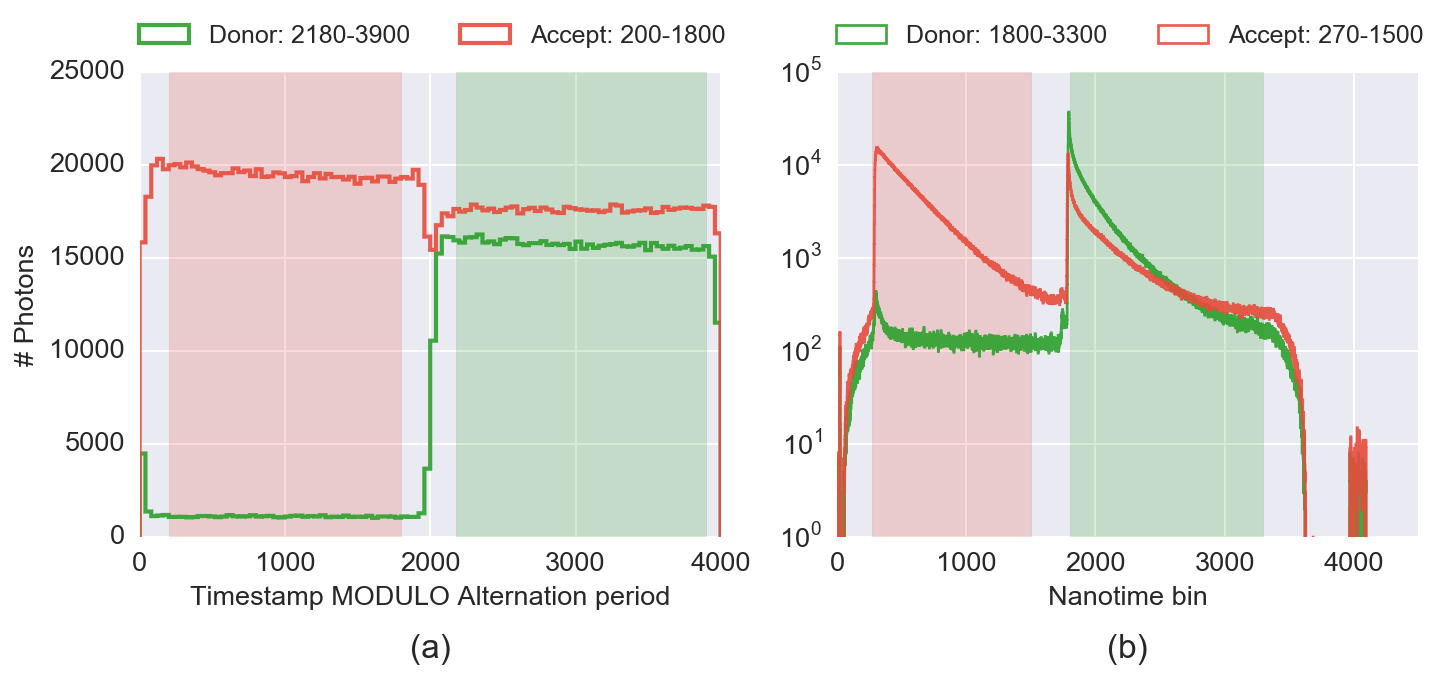
\includegraphics[width=1\columnwidth]{figures/ALEX_alternation_double/ALEX_alternation_double}
\caption{\label{fig:altern_hist_double}
\textbf{Alternation histograms for μs-ALEX and ns-ALEX measurements.}
Histograms used for the selection/determination
of the alternation periods for two typical smFRET-ALEX experiments.
Distributions of photons detected by donor channel are in \textit{green},
and by acceptor channel in \textit{red}.
The light \textit{green} and \textit{red} shaded areas indicate the donor
and acceptor period definitions.
(a) μs-ALEX alternation histogram, i.e. histogram of timestamps \textit{modulo}
the alternation period for a smFRET measurement.
(b) ns-ALEX TCSPC nanotime histogram for a smFRET measurement.
Both plots have been generated by the same plot function
(\texttt{plot\_alternation\_hist()}).
Additional information on these specific measurements can be found in the
attached notebook
(\href{http://nbviewer.jupyter.org/github/tritemio/fretbursts_paper/blob/master/notebooks/Figures\%20-\%20ALEX\%20histograms.ipynb}{link}).%
}
\end{center}
\end{figure}


To change the period definitions, we can type:

\begin{lstlisting}
d.add(D_ON=(2100, 3900), A_ON=(100, 1900))
\end{lstlisting}

where \verb|D_ON| and \verb|A_ON| are tuples (pairs of numbers) representing
the \textit{start} and \textit{stop} values for D or A excitation periods.
The previous command works for both μs-ALEX and ns-ALEX measurements.
After changing the parameters, a new alternation plot will show the updated
period definitions.

The alternation period definition can be applied to the data
using the function \verb|loader.alex_apply_period|
(\href{http://fretbursts.readthedocs.org/en/latest/loader.html#fretbursts.loader.alex_apply_period}{link}):

\begin{lstlisting}
loader.alex_apply_period(d)
\end{lstlisting}

After this command, \verb|d| will contain only photons inside the defined excitation periods.
If the user needs to update the periods definition, the data file will need to be
reloaded and the steps above repeated as described.


\subsection*{Background Estimation}
\label{sec:bg_calc}

The first step of smFRET analysis involves estimating background rates.
For example, to compute the background every 30~s, using a minimal inter-photon
delay fixed threshold of 2~ms for the all photon streams, the corresponding command is:

\begin{lstlisting}
d.calc_bg(bg.exp_fit, time_s=30, tail_min_us=2000)
\end{lstlisting}

The first argument (\verb|bg.exp_fit|) is the function used to fit the
background rate for each photon stream (see section~\nameref{sec:bg_intro}).
The function
\verb|bg.exp_fit| estimates the background using a maximum likelihood estimation
(MLE) of the delays distribution.
The second argument, \verb|time_s|, is the duration of the
\textit{background period} (section~\nameref{sec:bg_intro}) and the third, \verb|tail_min_us|,
is the minimum inter-photon delay to use when fitting the distribution to the specified model function.
To use different thresholds for each photon stream we pass a
tuple (i.e. a comma-separated list of values, \href{https://docs.python.org/3.5/tutorial/datastructures.html#tuples-and-sequences}{link}) instead of a scalar.
The recommended approach is however automating the choice of threshold using
\verb|tail_min_us='auto'| using an heuristic algorithm which is described in
\textit{Background estimation} section of the μs-ALEX tutorial
(\href{http://nbviewer.jupyter.org/github/tritemio/FRETBursts_notebooks/blob/master/notebooks/FRETBursts%20-%20us-ALEX%20smFRET%20burst%20analysis.ipynb#Background-estimation}{link}).
Finally, it is possible to use a slower but rigorous approach for finding the optimal
threshold as described in~\nameref{sec:bg_opt_th}. % SI_link

FRETBursts provides two kinds of plots to represent the background. One shows the histograms
of inter-photon delays compared to the fitted exponential distribution, shown in
figure~\ref{fig:bg_dist_all}) (see section~\nameref{sec:bg_intro} for details on the inter-photon distribution).
This plot is created with the command:

\begin{lstlisting}
dplot(d, hist_bg, period=0)
\end{lstlisting}

This command reflects the general form of plotting commands in FRETBursts
as described in~\nameref{sec:plotting}. % SI_link
Here we only note that the argument \verb|period| is an integer specifying the background
period to be plotted (when omitted, the default is 0, i.e. the first period).
Figure~\ref{fig:bg_dist_all} allows to quickly identify pathological cases where the
background fitting procedure returns unreasonable values.

The second background-related plot represents a timetrace of background rates,
as shown in figure~\ref{fig:bg_timetrace}. This plot allows monitoring background rate variations
occurring during the measurement and is obtained with the command:

\begin{lstlisting}
dplot(d, timetrace_bg)
\end{lstlisting}

Normally, samples should have a fairly constant background rate as a function of time
as in figure~\ref{fig:bg_timetrace}(a). However, sometimes, non-ideal
experimental conditions can yield a time-varying background rate, as illustrated in
figure~\ref{fig:bg_timetrace}(b).
A possible reason for the observed behavior could be buffer evaporation from an open sample
or poorly sealed observation chamber. Additionally,
cover-glass impurities can contribute to the background.
These impurities tend to bleach on timescales of minutes resulting in
background variations during the course of the measurement.

\paragraph*{Python details}

The estimated background rates are stored in the \verb|Data| attributes
\verb|bg_dd|, \verb|bg_ad| and \verb|bg_aa|, corresponding to photon
streams \verb|Ph_sel(Dex='Dem')|, \verb|Ph_sel(Dex='Aem')| and \verb|Ph_sel(Aex='Aem')|
respectively.
These attributes are lists of arrays (one array per excitation spot).
The arrays contain the estimated background rates in the different time windows
(background periods).
Additional background fitting functions (e.g. least-square fitting of inter-photon delay
histogram) are available in \verb|bg| namespace
(i.e. the \verb|background| module,
\href{http://fretbursts.readthedocs.org/en/latest/background.html}{link}).


\subsection*{Burst Search}
\label{sec:burstsearch}

%\subsubsection*{Burst Search in FRETBursts}
%\label{sec:burstsearch_code}

Following background estimation, burst search is the next step of
the analysis.
In FRETBursts, a standard burst search using a single photon stream
(see section~\nameref{sec:burstsearch_intro}) is performed by calling the
\verb|Data.burst_search| method
(\href{http://fretbursts.readthedocs.org/en/latest/data_class.html#fretbursts.burstlib.Data.burst_search}{link}).
For example, the following command:

\begin{lstlisting}
d.burst_search(F=6, m=10, ph_sel=Ph_sel('all'))
\end{lstlisting}

performs a burst search on all photons
(\verb|ph_sel=Ph_sel('all')|), with a count rate threshold equal to 6 times the
local background rate (\verb|F=6|), using 10 consecutive photons to compute the
local count rate (\verb|m=10|).
A different photon stream, threshold ($F$) or number of photons $m$ can be selected
by passing different values.
These parameters are good general-purpose starting point for smFRET analysis
but can they can be adjusted if needed.

Note that the previous burst search does not perform any burst size selection
(however, by definition, the minimum bursts size is effectively $m$).
An additional parameter $L$ can be passed to impose a minimum burst
size before any correction.
However, it is recommended to select bursts only after background corrections
are applied, as discussed in the next section~\nameref{sec:burstsel}.

It might sometimes be useful to specify a fixed photon-rate threshold, instead
of a threshold depending on the background rate, as in the previous example. In
this case, instead of $F$, the argument \verb|min_rate_cps| can be used to
specify the threshold (in counts-per-second). For example, a burst search with
a 50~kcps threshold is performed as follows:

\begin{lstlisting}
d.burst_search(min_rate_cps=50e3, m=10,
               ph_sel=Ph_sel('all'))
\end{lstlisting}

Finally, to perform a DCBS burst search (or in general an AND gate burst search,
see section~\nameref{sec:burstsearch_intro}) we use the function
\verb|burst_search_and_gate|
(\href{http://fretbursts.readthedocs.org/en/latest/plugins.html#fretbursts.burstlib_ext.burst_search_and_gate}{link}),
as illustrated in the following example:

\begin{lstlisting}
d_dcbs = bext.burst_search_and_gate(d, F=6, m=10)
\end{lstlisting}

The last command puts the burst search results in a new copy of the \verb|Data| variable \verb|d|
(in this example, the copy is called \verb|d_dcbs|).
Since FRETBursts shares the timestamps and detectors arrays between
different copies of \verb|Data| objects, the memory usage is minimized, even when
several copies are created.

\paragraph*{Python details}
Note that, while \verb|.burst_search()| is a method of \verb|Data|,
\verb|burst_search_and_gate| is a function in the \verb|bext| module
taking a \verb|Data| object as a first argument and returning a new
\verb|Data| object.

The function \verb|burst_search_and_gate| accepts optional arguments,
\verb|ph_sel1| and \verb|ph_sel2|, whose default values correspond to the
classical DCBS photon stream selection (see section~\nameref{sec:burstsearch_intro}).
These arguments can be specified to select different photon streams than those used in
a classical DCBS.

The \verb|bext| module (\href{http://fretbursts.readthedocs.org/en/latest/plugins.html}{link})
collects ``plugin'' functions that provides additional algorithms
for processing \verb|Data| objects.

\subsection*{Bursts Corrections}
\label{sec:corrcoeff}

In μs-ALEX, there are 3 important correction parameters: $\gamma$-factor,
donor leakage into the acceptor channel
and acceptor direct excitation by the donor excitation laser~\cite{Lee_2005}.
These corrections can be applied to burst data by simply assigning values
to the respective \verb|Data| attributes:

\begin{lstlisting}
d.gamma = 0.85
d.leakage = 0.15
d.dir_ex = 0.08
\end{lstlisting}

These attributes can be assigned either before or after the burst search. In the
latter case, existing burst data is automatically updated using the new
correction parameters.

These correction factors can be used to display corrected FRET distributions.
However, when the goal is to fit the FRET efficiency of sub-populations,
it is simpler to fit the background-corrected
PR histogram and then correct the population-level PR value (see SI in~\cite{Lee_2005}).
Correcting PR of each population (instead of correcting the data in each burst)
avoids distortion of the FRET distribution and keeps peaks of
static FRET subpopulations closer to the ideal Binomial statistics~\cite{Gopich_2007}.

FRETBursts implements the correction formulas for $E$ and $S$ in the functions
\verb|fretmath.correct_E_gamma_leak_dir| and \verb|fretmath.correct_S|
(\href{http://fretbursts.readthedocs.org/en/latest/fretmath.html}{link}).
A derivation of these correction formulas (using computer-assisted algebra)
can be found online as an interactive notebook (\href{http://nbviewer.jupyter.org/github/tritemio/notebooks/blob/master/Derivation%20of%20FRET%20and%20S%20correction%20formulas.ipynb}{link}).


\subsection*{Burst Selection}
\label{sec:burstsel}

After burst search, it is common to select bursts according to different
criteria. One of the most common is burst size.

For instance, to select bursts with more than 30 photons detected during the donor excitation
(computed after background correction), we use following command:

\begin{lstlisting}
ds = d.select_bursts(select_bursts.size, th1=30)
\end{lstlisting}

The previous command creates a new \verb|Data| variable (\verb|ds|) containing
the selected bursts. \verb|th1| defines the lower bound for burst size, while
\verb|th2| defines the upper bound (when not specified, as in the previous example,
the upper bound is $+\infty$).
As before, the new object (\verb|ds|) will share the photon data
arrays with the original object (\verb|d|) in order to minimize the amount
of used memory.

The first argument of \verb|select_bursts|
(\href{http://fretbursts.readthedocs.org/en/latest/data_class.html#burst-selection-methods}{link})
is a python function implementing the ``selection rule'' (\verb|select_bursts.size| in this example);
all remaining arguments (only \verb|th1| in this case) are parameters of the selection rule.
The \verb|select_bursts| module
(\href{http://fretbursts.readthedocs.org/en/latest/burst_selection.html}{link})
contains numerous built-in selection functions
(\href{http://fretbursts.readthedocs.org/en/latest/burst_selection.html#module-fretbursts.select_bursts}{link}).
For example,
\verb|select_bursts.ES|
is used to select a region on the E-S ALEX histogram,
\verb|select_bursts.width|
to select bursts based on their duration.
New custom criteria can be readily implemented by defining a new selection function,
which requires only a couple of lines of code (see the
\verb|select_bursts| module's source code for examples,
\href{https://github.com/tritemio/FRETBursts/blob/master/fretbursts/select_bursts.py}{link}).

Finally, different criteria can be combined sequentially.
For example, with the following commands:

\begin{lstlisting}
ds = d.select_bursts(select_bursts.size,
                     th1=50, th2=200)
dsw = ds.select_bursts(select_bursts.width,
                       th1=0.5e-3, th2=3e-3)
\end{lstlisting}

bursts in \verb|dsw|
will have sizes between 50 and 200 photons, and duration between 0.5 and 3~ms.

\paragraph*{Burst Size Selection}
In the previous section, we selected bursts by size, using only
photons detected in both D and A channels during D excitation (i.e. Dex photons),
as in eq.~\ref{eq:burstsize_dex}.
Alternatively, a threshold on the burst size computed including all photons
can be applied by adding $n_{aa}$ to the burst size (see eq.~\ref{eq:burstsize_allph}).
This is achieved
by passing \verb|add_naa=True| to the selection function.
The complete selection command is:

\begin{lstlisting}
ds = d.select_bursts(select_bursts.size,
                     th1=30, add_naa=True)
\end{lstlisting}

\noindent The result of this selection is plotted in figure~\ref{fig:alex_jointplot}.
When \verb|add_naa| is not specified,
as in the previous section, the default is \verb|add_naa=False|
(i.e. compute size using only Dex photons).

\begin{figure}[h!]
\begin{center}
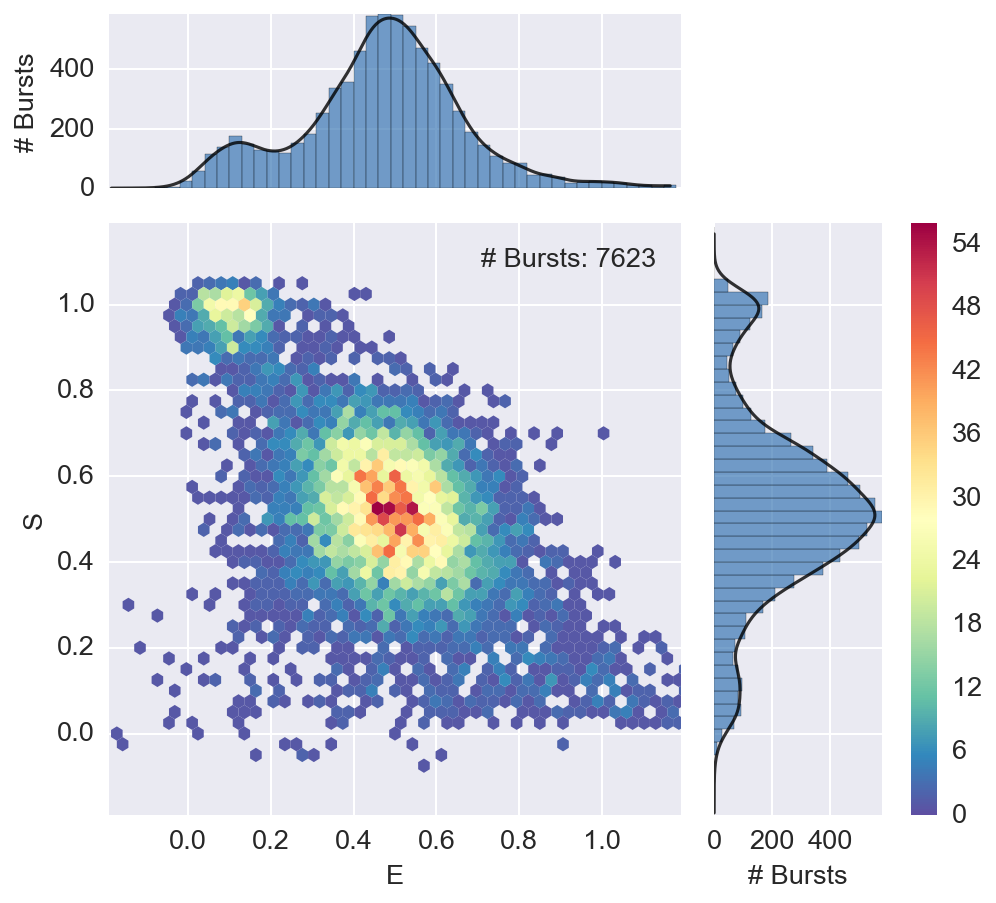
\includegraphics[width=0.7\columnwidth]{figures/alex_jointplot/alex_jointplot}
\caption{\label{fig:alex_jointplot} \textbf{E-S histogram showing FRET, D-only and A-only populations.}
A 2-D ALEX histogram and marginal E and S histograms for a 40-bp dsDNA
with D-A distance of 17 bases (Donor dye: ATTO550, Acceptor dye: ATTO647N).
Bursts are selected with a size-threshold of 30 photons, including Aex photons.
The plot is obtained with \texttt{alex\_jointplot(ds)}. The 2D E-S distribution plot (join plot)
is an histogram with hexagonal bins, which reduce the binning artifacts (compared to square bins)
and naturally resembles a scatter-plot when the burst density is low.
Three populations are visible: FRET population (middle), D-only population (top left) and
A-only population (bottom, $S < 0.2$). Compare with figure~\ref{fig:alex_jointplot_fretsel}
where the FRET population has been isolated.%
}
\end{center}
\end{figure}


Another important parameter for defining the burst size is the $\gamma$-factor, i.e.
the imbalance between the donor and the acceptor channel signals. As noted in
section~\nameref{sec:burstsizeweights}, the $\gamma$-factor is
used to compensate bias for the different fluorescence quantum yields of the D and A
fluorophores as well as the different photon-detection efficiencies of the D and A channels.
When $\gamma$ is significantly different from 1, neglecting its effect on burst size leads to
over-representing (in terms of number of bursts) one FRET population versus the others.

When the $\gamma$ factor is known, a more unbiased selection of different FRET
populations can be achieved passing the argument \verb|gamma| to the
selection function:

\begin{lstlisting}
ds = d.select_bursts(select_bursts.size,
                     th1=15, gamma=0.65)
\end{lstlisting}

When not specified, $\gamma=1$ is assumed.

For more details on burst size selection, see the
\verb|select_bursts.size| documentation
(\href{http://fretbursts.readthedocs.org/en/latest/burst_selection.html#fretbursts.select_bursts.size}{link}).

\paragraph*{Python details}
To compute $\gamma$-corrected burst sizes (with or without addition of \verb|naa|)
the method \verb|Data.burst_sizes|
(\href{http://fretbursts.readthedocs.org/en/latest/data_class.html#fretbursts.burstlib.Data.burst_sizes}{link})
is used.

\paragraph*{Select the FRET Populations}

In smFRET-ALEX experiments, in addition to one or more FRET populations, there are always
donor-only (D-only) and acceptor-only (A-only) populations.
In most cases, these additional populations are not of interest and need to be filtered out.

In principle, using the E-S representation, D-only and A-only bursts
can be excluded by selecting bursts within a range of $S$ values (e.g. S=0.2-0.8).
This approach, however, simply truncates the burst distribution with arbitrary
thresholds and is therefore not recommended for quantitative assessment of FRET
populations.

An alternative approach consists in applying two selection filters sequentially.
First, the A-only population is filtered out
by applying a threshold on the number of photons during D excitation (Dex).
Second, the D-only population is filtered out by applying a threshold on
the number of A photons during A excitation (AexAem).
The commands for these combined selections are:

\begin{lstlisting}
ds1 = d.select_bursts(select_bursts.size, th1=15)
ds2 = ds1.select_bursts(select_bursts.naa, th1=15)
\end{lstlisting}

Here, variable \verb|ds2| contains the combined burst selection.
Figure~\ref{fig:alex_jointplot_fretsel} shows the resulting pure FRET
population obtained with the previous selection.


\begin{figure}[h!]
\begin{center}
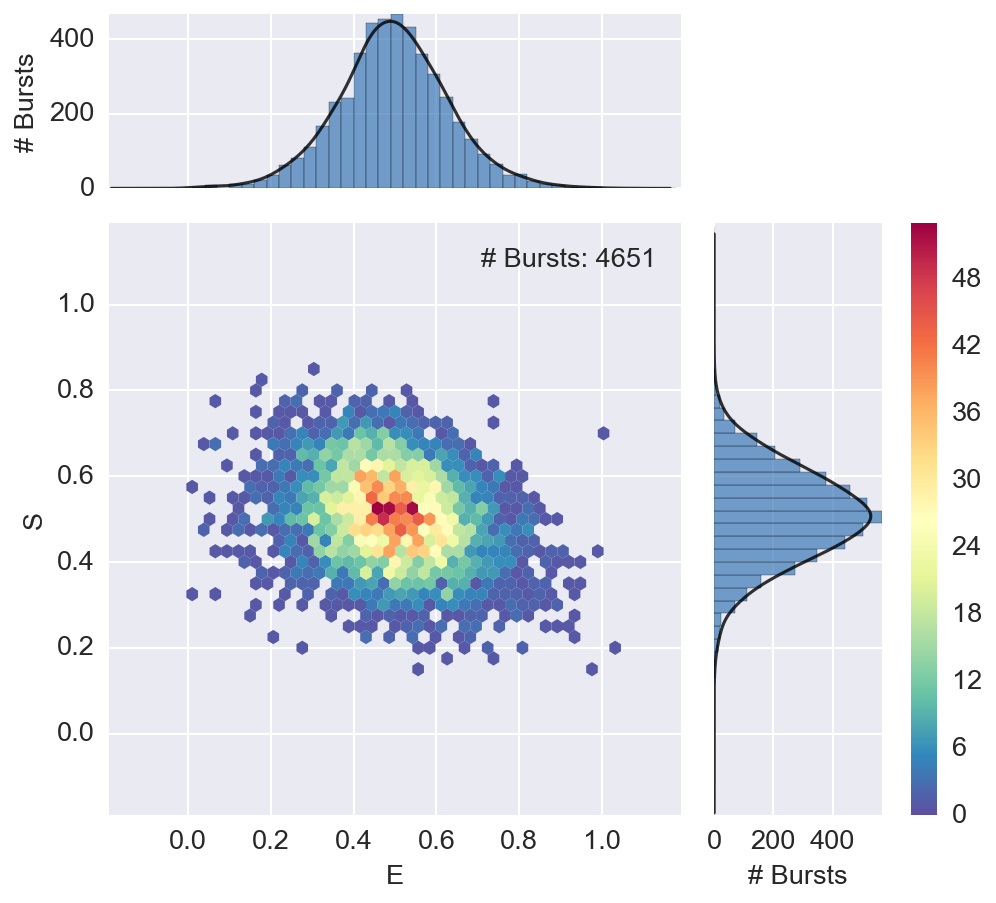
\includegraphics[width=0.7\columnwidth]{figures/alex_jointplot_fretsel/alex_jointplot_fretsel}
\caption{\label{fig:alex_jointplot_fretsel}
\textbf{E-S histogram after filtering out D-only and A-only populations.}
2-D ALEX histogram after selection of FRET population
using the composition of two burst selection filters:
(1) selection of bursts with counts in Dex stream larger than 15;
(2) selection of bursts with counts in AexAem stream larger than 15.
Compare to figure~\ref{fig:alex_jointplot} where all burst populations
(FRET, D-only and A-only) are reported.%
}
\end{center}
\end{figure}

\subsection*{Population Analysis}
\label{sec:fretfit}

Typically, after bursts selection, E or S histograms are fitted to a model.
FRETBursts \verb|mfit| module allows fitting histograms of bursts quantities
(i.e. E or S) with arbitrary models. In this context, a model is an object
specifying a function, the parameters varied during the fit
and optional constraints for these parameters. This concept of model
is taken from \textit{lmfit}~\cite{lmfit}, the underlying library used by
FRETBursts to perform the fits.

Models can be created from arbitrary functions. 
FRETBursts includes predefined (i.e. built-in) models 
such as 1 to 3 Gaussian peaks or 2-Gaussian connected by a flat plateau.
The latter is an empirical model that
can be used to more accurately fit the center values of two populations
when the peaks are connected by intermediate-FRET bursts
(for the analytical definition of this function see the documentation, 
\href{http://fretbursts.readthedocs.io/en/latest/mfit.html#fretbursts.mfit.factory_two_gaussians}{link}).
Built-in models are created by calling a corresponding factory function
(whose names start with \verb|mfit.factory_|) which initializes the parameters
with values and constraints suitable for E and S histograms fits.
(see \textit{Factory Functions} documentation,
\href{http://fretbursts.readthedocs.org/en/latest/mfit.html#model-factory-functions}{link}).

As an example, we can fit the E histogram of bursts in the
\verb|ds| variable with two Gaussian peaks with the following command:

\begin{lstlisting}
bext.bursts_fitter(ds, 'E', binwidth=0.03,
                   model=mfit.factory_two_gaussians())
\end{lstlisting}

Changing \verb|'E'| with \verb|'S'| will fit the S histogram instead.
The \verb|binwidth| argument specifies the histogram bin width and
the \verb|model| argument defines which model shall be used for
fitting.

All fitting results (including best fit values, uncertainties, etc...),
are stored in the \verb|E_fitter| (or \verb|S_fitter|)
attributes of the \verb|Data| variable (named \verb|ds| here).
To print a comprehensive summary of the fit results, including
uncertainties, reduced $\chi^2$ and correlation between parameters,
the we use the following command:

\begin{lstlisting}
fit_res = ds.E_fitter.fit_res[0]
print(fit_res.fit_report())
\end{lstlisting}

Finally, to plot the fitted model together with the FRET histogram,
as shown in figure~\ref{fig:histfit}, we pass the parameter \verb|show_model=True|
to the \verb|hist_fret| function as follows
(see~\nameref{sec:plotting} for an introduction to plotting in FRETBursts):

\begin{lstlisting}
dplot(ds, hist_fret, show_model=True)
\end{lstlisting}


\begin{figure}[h!]
\begin{center}
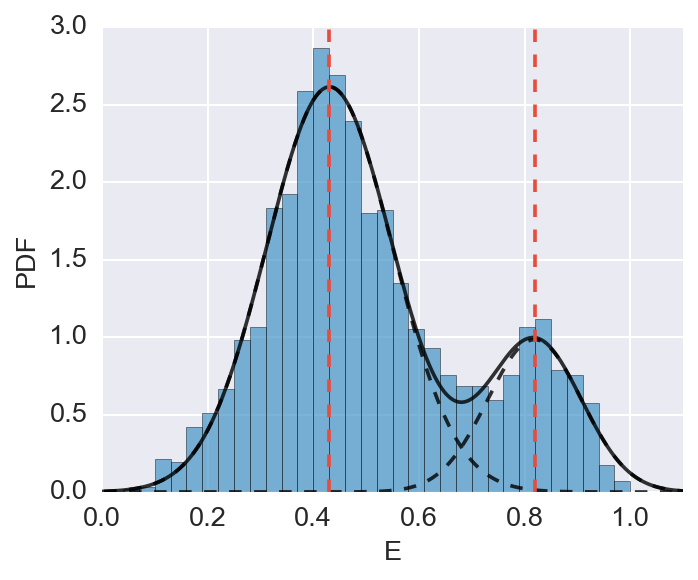
\includegraphics[width=0.49\columnwidth]{figures/hist_fit/hist_fit}
\caption{\label{fig:histfit} \textbf{FRET histogram fitted with two Gaussians.}
Example of a FRET histogram fitted with a 2-Gaussian model.
After performing the fit (see main text), the plot is generated
with \texttt{dplot(ds, hist\_fret, show\_model=True)}.%
}
\end{center}
\end{figure}

For more examples on fitting bursts data and plotting results, refer to the
fitting section of the μs-ALEX notebook (\href{http://nbviewer.jupyter.org/github/tritemio/FRETBursts_notebooks/blob/master/notebooks/FRETBursts%20-%20us-ALEX%20smFRET%20burst%20analysis.ipynb#FRET-fit:-in-depth-example}{link}),
the \textit{Fitting Framework} section of the documentation
(\href{http://fretbursts.readthedocs.org/en/latest/fit.html}{link})
as well as the documentation for \verb|bursts_fitter| function
(\href{http://fretbursts.readthedocs.org/en/latest/plugins.html#fretbursts.burstlib_ext.bursts_fitter}{link}).

\paragraph*{Python details}

Models returned by FRETBursts's factory functions (\verb|mfit.factory_*|)
are \verb|lmfit.Model| objects (\href{https://lmfit.github.io/lmfit-py/model.html}{link}).
Custom models can be created by calling \verb|lmfit.Model| directly.
When an \verb|lmfit.Model| is fitted, it returns a \verb|ModelResults| object
(\href{https://lmfit.github.io/lmfit-py/model.html#the-modelresult-class}{link}),
which contains all information related to the fit (model, data,
parameters with best values and uncertainties) and useful methods to operate on fit results.
FRETBursts puts a \verb|ModelResults| object of each excitation spot in the list
\verb|ds.E_fitter.fit_res|.
For instance, to obtain the reduced $\chi^2$ value of the E histogram fit in a
single-spot measurement \verb|d|, we use the following command:

\begin{lstlisting}
d.E_fitter.fit_res[0].redchi
\end{lstlisting}

Other useful attributes are \verb|aic| and \verb|bic| which contain
respectively the Akaike information criterion (AIC)~\cite{akaike_new_1974} 
and the Bayes Information criterion (BIC)~\cite{schwarz_estimating_1978}.
AIC and BIC are general-purpose statistical criteria for comparing 
models and selecting the most appropriate for a given dataset.
By penalizing models with higher number of parameters, these criteria 
strike a balance between the need of achieving high goodness of fit 
with the need of keeping the model complexity low to avoid overfitting.

Examples of definition and modification of fit models are provided in
the aforementioned μs-ALEX notebook
(\href{http://nbviewer.jupyter.org/github/tritemio/FRETBursts_notebooks/blob/master/notebooks/FRETBursts%20-%20us-ALEX%20smFRET%20burst%20analysis.ipynb#FRET-fit:-in-depth-example}{link}).
Users can also refer to the comprehensive lmfit's documentation
(\href{http://lmfit.github.io/lmfit-py/}{link}).

\subsection*{FRET Dynamics}
\label{sec:dynamics}

FRET peaks resolved from FRET histograms correspond to different FRET
populations. However determining whether these populations are due to static
heterogeneity (different D-A distances, Förster radius, etc.) or a
dynamic equilibrium, requires further analysis.

Shot-noise analysis (SNA)~\cite{Nir_2006} or probability
distribution analysis (PDA)~\cite{Antonik2006} allow to compute
the minimal width of a FRET peak originating from a single
FRET efficiency. Typically, several mechanisms
contribute to the broadening of the experimental FRET peak
beyond the shot-noise limit. For example, heterogeneities in the sample
(resulting in a distribution of Förster radiuses)
or actual conformational changes (resulting in a distribution
of D-A distances) can cause FRET peak broadening~\cite{sisamakis_accurate_2010}.

Kalinin~\cite{Kalinin2010} and Santoso~\cite{santoso_probing_2009}
extended the PDA approach to estimate conversion rates between different
states by comparing FRET histograms as a function of the time-bin size.
Gopich and Szabo~\cite{Gopich2009, gopich_theory_2011} developed
a related method to compute conversion rates using
a likelihood function which depends on photon timestamps (overcoming
the time binning and FRET histogramming step).
Hoffman~\cite{hoffmann_quantifying_2011} proposed a method 
called RASP (recurrence analysis of single particles) to extend 
the timescale of detectable kinetics.
Hoffman computes the probability that two nearby bursts are originating from
the same molecule and therefore allows to set a time-threshold
for considering consecutive bursts as originating from the same molecule.

Other two related methods for discriminating between static heterogeneity
and sub-millisecond dynamics are Burst Variance Analysis
(BVA) proposed by Torella~\cite{Torella_2011} and
kernel density distribution estimator (2CDE) proposed by 
Tomov~\cite{Tomov_2012}. The latter method computes local
photon rates from timestamps within bursts using
Kernel Density Estimation (KDE)
(FRETBursts includes general-purpose functions
to compute KDE of photon timestamps in the \verb|phrates| module, 
(\href{http://fretbursts.readthedocs.io/en/latest/phrates.html}{link})).

The BVA and 2CDE methods are implemented 
in two notebooks included with FRETBursts
(\href{http://nbviewer.jupyter.org/github/tritemio/FRETBursts_notebooks/blob/master/notebooks/Example%20-%20Burst%20Variance%20Analysis.ipynb}{BVA link},
\href{http://nbviewer.jupyter.org/github/tritemio/FRETBursts_notebooks/blob/master/notebooks/Example%20-%202CDE%20Method.ipynb}{2CDE link}).
To use them, a user needs to download the relevant notebook
and run the anaysis therein.
The other methods mentioned in this section are not currently 
implemented in FRETBursts.
However, users can implement their additional favorite method
taking advantage of FRETBursts functions for burst analysis
and timestamps/bursts manipulation.
To facilitate this task, in the next section,
we show how to perform low-level analysis of timestamps and bursts data 
by implementing the BVA method from scratch.
An additional example showing how to split bursts in constant time-bins
can be found in the respective FRETBursts notebook
(\href{http://nbviewer.jupyter.org/github/tritemio/FRETBursts_notebooks/blob/master/notebooks/Example%20-%20Working%20with%20timestamps%20and%20bursts.ipynb}{link}).
These examples serve as a guide for implementing new methods.
We welcome researchers willing to implement new methods to ask questions
on GitHub or on the mailing list. 
We also encourage sharing eventual new methods implemented in FRETBursts 
for the benefit the entire community.


\section*{Implementing Burst Variance Analysis}

\label{sec:bva}
In this section, we describe how to implement burst variance analysis (BVA)
as described in~\cite{Torella_2011}.
FRETBursts provides well-tested, general-purpose functions for timestamps and burst data
manipulation and therefore simplifies implementing custom burst analysis algorithms such as BVA.

\subsection*{BVA Overview}
Single-molecule FRET histograms show more information than just mean FRET efficiencies.
While in general the presence of several peaks clearly indicates the existence of
multiple subpopulations, a single peak cannot a priori be associated with
a single population defined by a unique FRET efficiency without further analysis
(such as, for instance, shot-noise analysis~\cite{Nir_2006,Antonik2006}).

The FRET histogram of a single FRET population has a minimum width set by shot noise
(i.e. the width is caused by the statistics of discrete photon-detection events).
FRET distributions broader than the shot noise limit,
can be ascribed to either a static mixture of species with slightly different FRET efficiencies,
or to a specie undergoing dynamic transitions (e.g. interconversion between multiple states,
diffusion in a continuum of conformations, binding-unbinding events, etc.).
When the single peak of a FRET distribution is wider than predicted from shot-noise,
it is not possible to discriminate between the static and dynamic case without further analysis.
The BVA method has been developed to address this issue, namely identifying the presence of dynamics
in FRET distributions~\cite{Torella_2011},
and has been successfully applied to identify biomolecular processes with
dynamics on the millisecond time-scale~\cite{Torella_2011, Robb_2013}.

The basic idea behind BVA is to subdivide bursts into contiguous burst chunks (sub-bursts)
comprising a fixed number $n$ of photons,
and to compare the empirical variance of acceptor counts of all sub-bursts in a burst,
with the theoretical shot-noise-limited variance.
An empirical variance of sub-bursts larger than the shot-noise limited value indicates
the presence of dynamics. Since the estimation of the sub-bursts variance is affected
by uncertainty, BVA analysis provides and indication of an higher or lower probability
of observing dynamics.

In a FRET (sub-)population originating from a single static FRET efficiency,
the sub-bursts acceptor counts $n_a$ can be modeled as a binomial-distributed random variable
$N_a \sim \operatorname{B}(n, E_p)$, where $n$ is the number of photons in each sub-burst and
$E_p$ is the estimated population proximity-ratio (PR).
Note that we can use the PR because, regardless of the molecular FRET efficiency,
the detected counts are partitioned between donor and acceptor channels according to
a binomial distribution with success probability equal to the PR.
The only approximation done here is neglecting the presence of background
(a reasonable approximation since the backgrounds counts are in general a
very small fraction of the total counts).
We refer the interested reader to~\cite{Torella_2011} for further discussion.

If $N_a$ follows a binomial distribution, the random variable $E_{\textrm{sub}} = N_a/n$,
has a standard deviation reported in eq.~\ref{eq:binom_std}.

\begin{equation}
\label{eq:binom_std}
\operatorname{Std}(E_{\textrm{sub}}) = \left( \frac{E_p\,(1 - E_p)}{n} \right)^{1/2}
\end{equation}

BVA analysis consists of four steps: 1) dividing bursts into consecutive sub-bursts
containing a constant number of consecutive photons~\textit{n}, 2) computing the PR
of each sub-burst, 3) calculating the empirical standard deviation ($s_E$) of sub-bursts
PR in each burst, and 4) comparing $s_E$ to the expected standard deviation
of a shot-noise-limited distribution~(eq.~\ref{eq:binom_std}).
If, as in figure~\ref{fig:bva_static}, the observed FRET efficiency distribution
originates from a static mixture of sub-populations (of different
non-interconverting molecules) characterized by distinct FRET efficiencies,
$s_E$ of each burst is only affected by shot-noise and will follow the expected
standard deviation curve based on eq.~\ref{eq:binom_std}.
Conversely, if the observed distribution originates from biomolecules belonging to a single specie,
which interconverts between different FRET sub-populations (over times comparable to the diffusion
time), as in figure~\ref{fig:bva_dynamic}, $s_E$ of each burst will be larger than the expected
shot-noise-limited standard deviation, and will be located above the shot-noise standard
deviation curve (right panel of figure~\ref{fig:bva_dynamic}).


\begin{figure}[h!]
\begin{center}
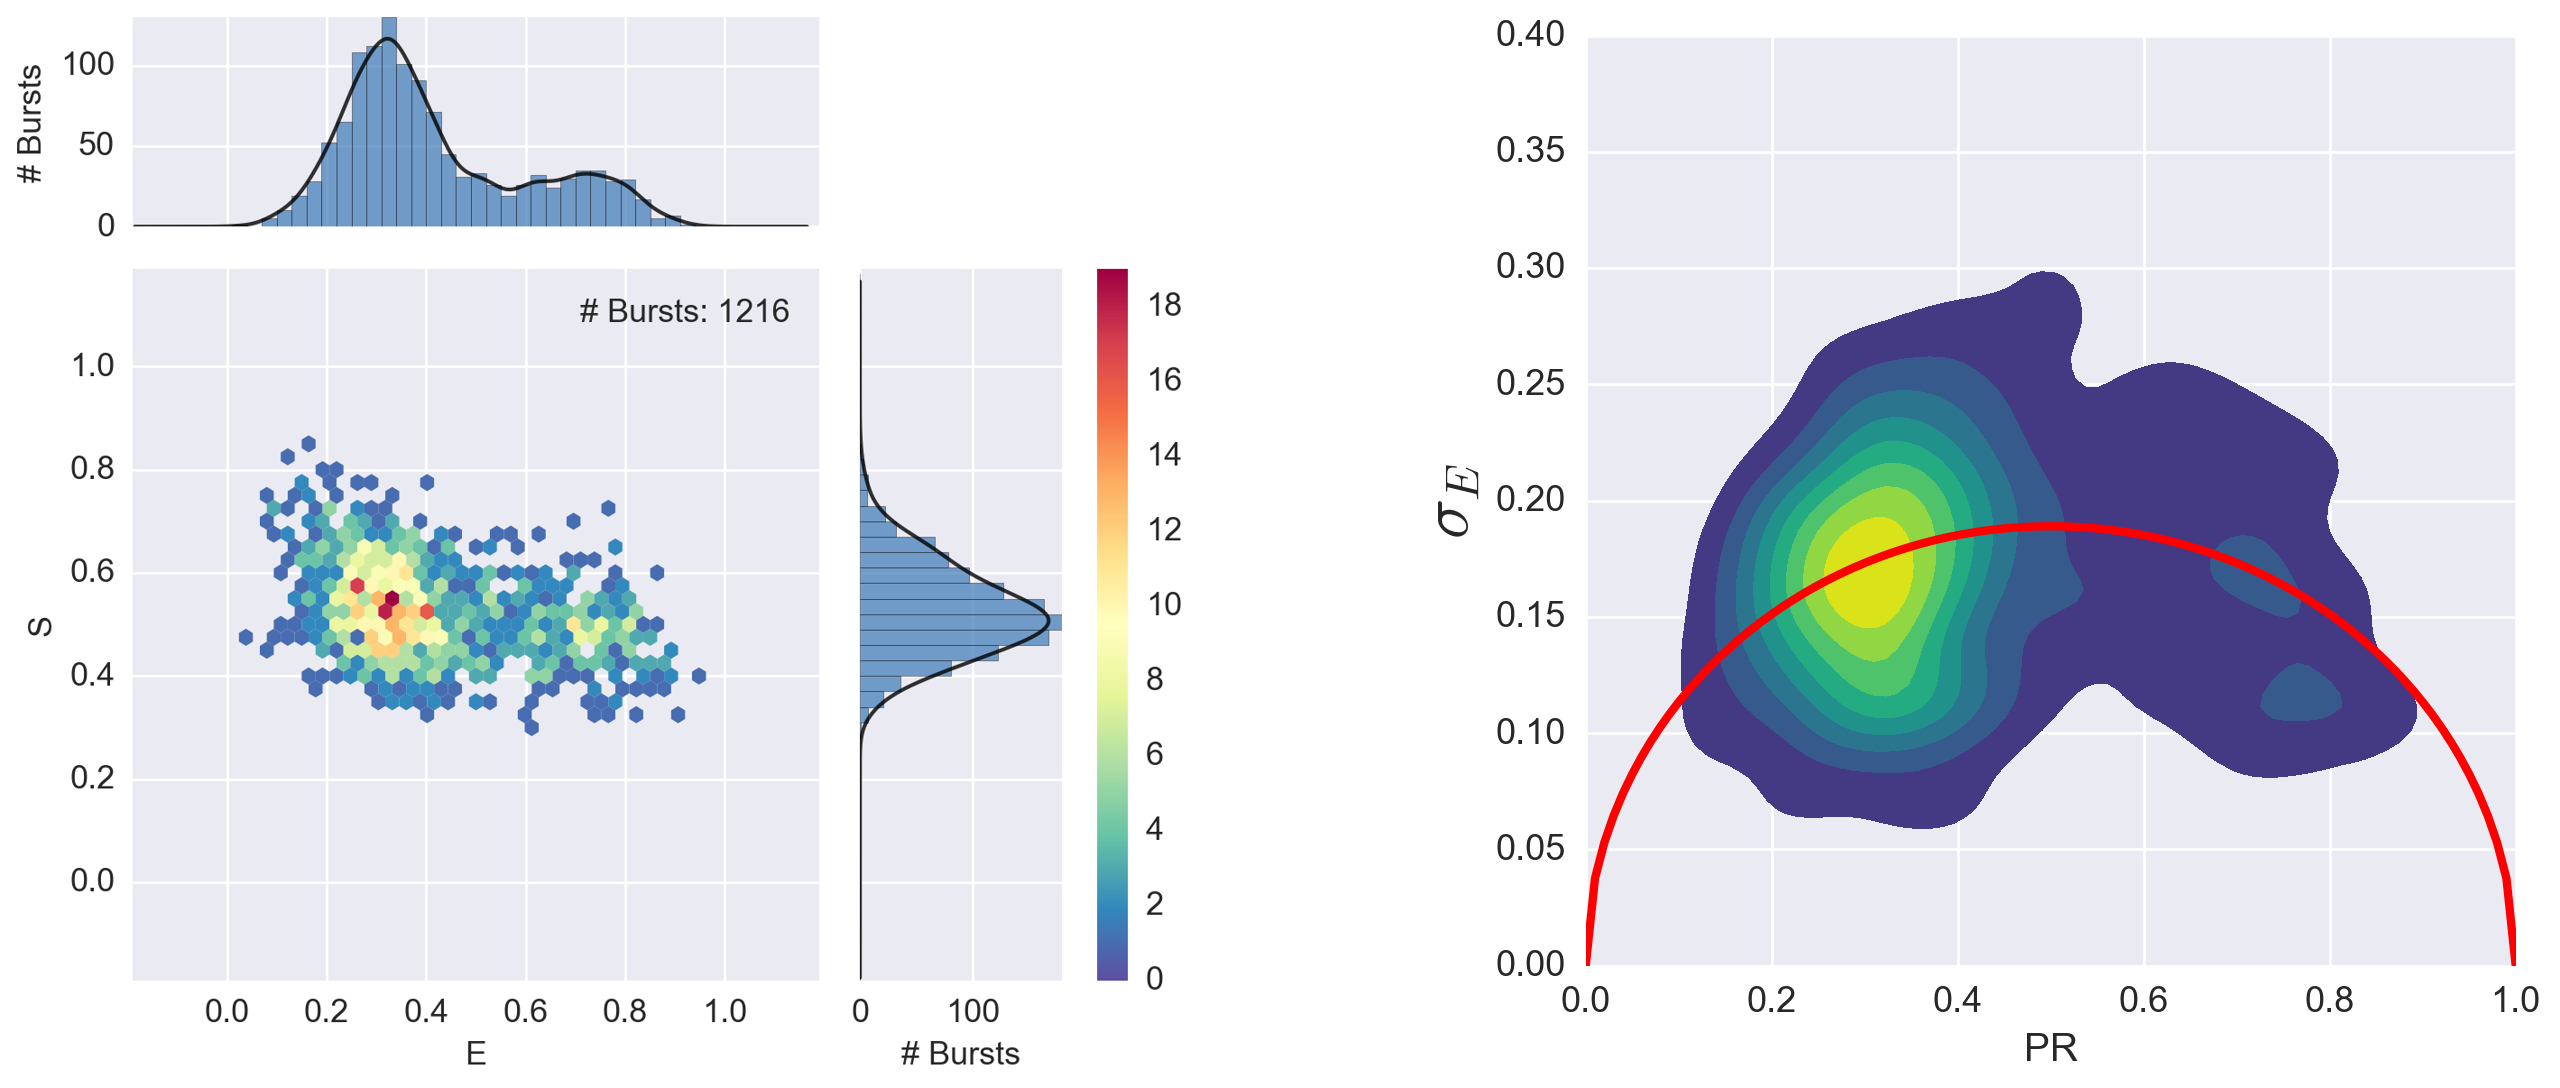
\includegraphics[width=0.98\columnwidth]{figures/ALEX_BVA_static/ALEX_BVA_static}
\caption{\label{fig:bva_static}  \textbf{BVA distribution for a static mixture sample.}
The left panel shows the E-S histogram for a mixture of single stranded DNA (20dT) and double stranded DNA (20dT-20dA) molecules in  200 mM MgCl$_2$. The right panel shows the corresponding BVA plot. Since both 20dT and 20dT-20dA are stable and have no dynamics, the BVA plots shows $s_E$ peaks lying on the static standard deviation curve (\textit{red curve}).%
}
\end{center}
\end{figure}

\begin{figure}[h!]
\begin{center}
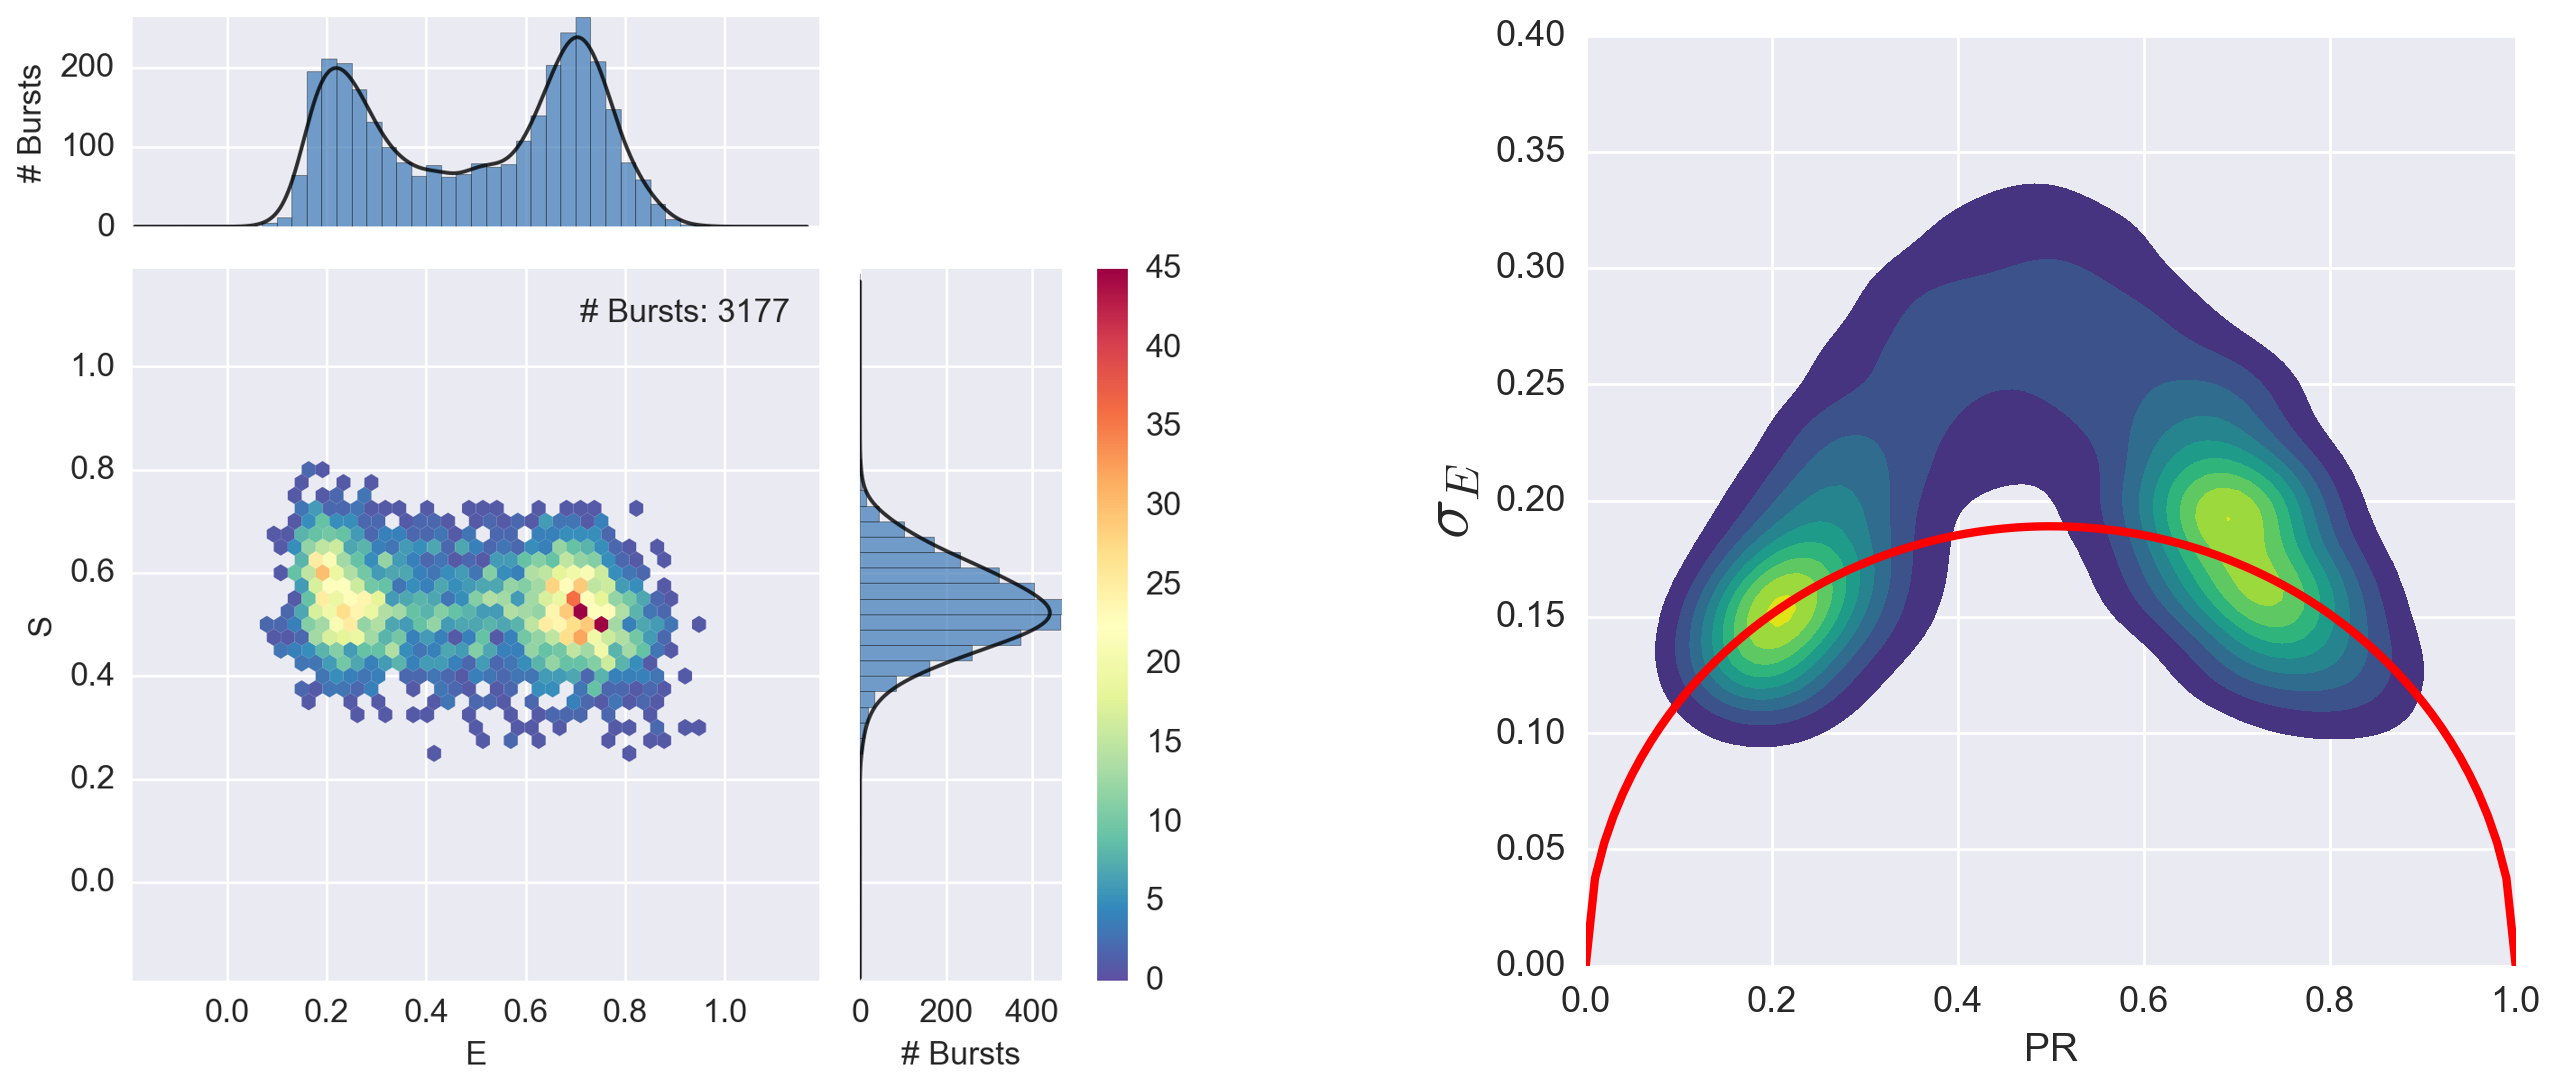
\includegraphics[width=0.98\columnwidth]{figures/ALEX_BVA_dynamic/ALEX_BVA_dynamic}
\caption{\label{fig:bva_dynamic} \textbf{BVA distribution for a hairpin sample undergoing dynamics.}
The left panel shows the E-S histogram for a single stranded DNA sample ($A_{31}$-TA, see in~\cite{Tsukanov_2013}), designed to form a transient hairpin in 400mM NaCl. The right panel shows the corresponding BVA plot. Since the transition between hairpin and open structure causes a significant change in FRET efficiency, $s_E$ lies largely above the static standard deviation curve (\textit{red curve}).%
}
\end{center}
\end{figure}

\subsection*{BVA Implementation}

The following paragraphs describe the low-level details involved in implementing the BVA using FRETBursts.
The main goal is to illustrate a real-world example of accessing and manipulating timestamps and burst data.
For a ready-to-use BVA implementation users can refer to the corresponding notebook included with FRETBursts
(\href{http://nbviewer.jupyter.org/github/tritemio/FRETBursts_notebooks/blob/master/notebooks/Example%20-%20Burst%20Variance%20Analysis.ipynb}{link}).

\paragraph*{Python details}
For BVA implementation, two photon streams are needed: all-photons during donor excitation (Dex)
and acceptor photons during donor excitation (DexAem).
These photon stream selections are obtained by computing boolean masks as follows
(see~\nameref{sec:burststimes}):

\begin{lstlisting}
Dex_mask = ds.get_ph_mask(ph_sel=Ph_sel(Dex='DAem'))
DexAem_mask = ds.get_ph_mask(ph_sel=Ph_sel(Dex='Aem'))
DexAem_mask_d = AemDex_mask[Dex_mask]
\end{lstlisting}

Here, the first two variables (\verb|Dex_mask| and \verb|DexAem_mask|)
select photon from the all-photons timestamps array,
while \verb|DexAem_mask_d|, selects A-emitted photons from the
array of photons emitted during D-excitation. As shown below,
the latter is needed to count acceptor photons in burst chunks.

Next, we need to express bursts start-stop data as indexes of the D-excitation photon stream
(by default burst start-stop indexes refer to all-photons timestamps array):

\begin{lstlisting}
ph_d = ds_FRET.get_ph_times(ph_sel=Ph_sel(Dex='DAem'))
bursts = ds_FRET.mburst[0]
bursts_d = bursts.recompute_index_reduce(ph_d)
\end{lstlisting}

Here, \verb|ph_d| contains the Dex timestamps, \verb|bursts| the original burst data and
\verb|bursts_d| the burst data with start-stop indexes relative to \verb|ph_d|.

Finally, with the previous variables at hand, the BVA algorithm
can be easily implemented by computing the $s_E$ quantity for each burst:

\begin{lstlisting}
n = 7
E_sub_std = []
for burst in bursts_d:
    E_sub = []
    startlist = range(burst.istart, burst.istop + 2 - n, n)
    stoplist = [i + n for i in startlist]
    for start, stop in zip(startlist, stoplist):
        A_D = DexAem_mask_d[start:stop].sum()
        E = A_D / n
        E_sub.append(E)
    E_sub_std.append(np.std(E_sub))
\end{lstlisting}

Here, \verb|n| is the BVA parameter defining the number of photons in each burst chunk.
The outer loop iterates through bursts, while the inner loop iterates through sub-bursts.
The variables \verb|startlist| and \verb|stoplist| are the list of start-stop indexes for
all sub-bursts in current burst.
In the inner loop, \verb|A_D| and \verb|E| contain the number of acceptor photons and
FRET efficiency for the current sub-burst. Finally, for each burst, the standard deviation
of \verb|E| is appended to the list \verb|E_sub_std|.

By plotting the 2D distribution of $s_E$ (i.e. \verb|E_sub_std|) versus the average (uncorrected) E
we obtain the BVA plots of figure~\ref{fig:bva_static} and~\ref{fig:bva_dynamic}.



\section*{Conclusions}
\label{sec:conclusions}

FRETBursts is an open source and openly developed (see~\nameref{sec:dev}) implementation % SI_link
of established smFRET burst analysis methods
made available to the single-molecule community.
It implements several novel concepts which improve the analysis results, such as
time-dependent background estimation, background-dependent burst search threshold,
burst weighting and $\gamma$-corrected burst size selection.
More importantly, FRETBursts provides a library of thoroughly-tested functions
for timestamps and burst manipulation, making it an ideal platform for
developing and comparing new analytical techniques.

We envision FRETBursts both as a state-of-the-art burst analysis
software as well as a platform for development and assessment of novel algorithms.
To underpin this envisioned role, FRETBursts is developed following modern
software engineering practices, such as DRY principle
(\href{http://en.wikipedia.org/wiki/Don\%27t_repeat_yourself}{link})
to reduce duplication and KISS principle
(\href{http://en.wikipedia.org/wiki/KISS_principle}{link})
to reduce over-engineering. Furthermore, to minimize the number software errors~\cite{Merali_2010,Soergel_2015},
we employ defensive programming~\cite{Prli__2012} which includes code readability,
unit and regression testing and continuous integration~\cite{Eglen_2016}.
Finally, being open source, any scientist can inspect the source code,
fix errors, adapt it to her own needs.

We believe that, in the single-molecule community,
standard open source software implementations, such as FRETBursts, can enhance
reliability and reproducibility of analysis and promote a faster adoption of novel methods,
while reducing the duplication of efforts among different groups.

\section*{Acknowledgments}
We thank Dr. Eyal Nir and Dr. Toma Tomov for support in the implementation of the 2CDE method.
This work was supported by National Institutes of Health (NIH)
grant R01-GM95904 and R01-GM069709. Dr. Weiss discloses equity in
Nesher Technologies and intellectual property used in the research
reported here. The work at UCLA was conducted in Dr. Weiss's Laboratory.

\section*{Supporting Information}


\paragraph*{S1 Appendix.}
\label{sec:notebook}
{\bf Notebook Workflow.} A description of the notebook workflow used by FRETBursts.

\paragraph*{S2 Appendix.}
\label{sec:dev}
{\bf Development and Contributions.} A description of development philosophy and techniques
as well as how to contribute to the FRETBursts project.

\paragraph*{S3 Appendix.}
\label{sec:burststimes}
{\bf Timestamps and Burst Data.} General concepts of how timestamps and
bursts data are stored and handled in FRETBursts.

\paragraph*{S4 Appendix.}
\label{sec:plotting}
{\bf Plotting \texttt{Data}.} A description of the syntax used to perform
plots in FRETBursts.

\paragraph*{S5 Appendix.}
\label{sec:bg_opt_th}
{\bf Background Estimation With Optimal Threshold.} A description of
the algorithm used by FRETBursts to compute the
optimal threshold for background estimation.

\paragraph*{S6 Appendix.}
\label{sec:burstweights_theory}
{\bf Burst Weights.} Theory underpinning the choice of using burst size
as weights for FRET estimation.

\nolinenumbers
\bibliography{bibliography/converted_to_latex.bib%
}

\end{document}
